\documentclass[UTF8,zihao=-4,a4paper]{ctexart}
\usepackage{amsmath,amssymb,bm}
\usepackage{booktabs,longtable,tabularx}
\usepackage{geometry}
\usepackage{graphicx}
\usepackage{float,caption,placeins,tikz}
\usetikzlibrary{arrows.meta,positioning,shapes.geometric}
\setCJKmainfont{SimSun}[AutoFakeBold=2]
\setCJKsansfont{Microsoft YaHei}[AutoFakeBold=2]
\newCJKfontfamily\titlefont{Microsoft YaHei}[AutoFakeBold=2]
\ctexset{section={format=\centering\sffamily\bfseries\zihao{4}},subsection={format=\sffamily\bfseries\zihao{-4}},subsubsection={format=\sffamily\bfseries\zihao{-4}}}
\captionsetup{font=small,labelsep=quad}
\setlength{\textfloatsep}{14pt plus 3pt minus 3pt}
\setcounter{topnumber}{1}\setcounter{bottomnumber}{1}\setcounter{totalnumber}{1}
\renewcommand{\topfraction}{0.65}\renewcommand{\textfraction}{0.30}
\renewcommand{\floatpagefraction}{0.85}
\usepackage{fvextra}
\geometry{left=2.5cm,right=2.5cm,top=2.5cm,bottom=2.5cm}
\setlength{\parindent}{2em}
\setlength{\parskip}{0pt}
\linespread{1.45}
\setlength{\tabcolsep}{4pt}
\setlength{\emergencystretch}{8em}
\newcommand{\dd}{\,\mathrm d}
\newcolumntype{Y}{>{\raggedright\arraybackslash}X}
\newcommand{\keywords}[1]{\par\noindent\textbf{关键词：}#1}
\begin{document}
\pagestyle{plain}\songti\zihao{-4}\sloppy
\begin{center}\titlefont\zihao{3}考虑变物性与收缩效应的\\药材非线性热湿传递模型\end{center}

\begin{abstract}
药材热风干燥存在表面失水快、内部响应滞后及后期传质受限等现象，仅用平均含水率难以判断全域是否达标。针对圆柱形药材，本文以温度和干基含水率为状态，建立变物性径向热湿传递模型，并在收缩条件下采用归一化材料坐标统一描述计算域。

针对问题1，使用题给预热物性及环境观测构造对流边界，采用圆环有限体积法求解温湿分布。1800秒时中心与表面温度分别为33.5753和36.7856摄氏度，表面含水率降至1.5103千克/千克，中心仍接近初值，体现出明显的径向传递滞后。

针对问题2和问题3，将附录3经验物性纳入全程模型，以浓度区间积分计算非线性界面扩散系数，并通过表面加密网格和隐式迭代解析低含水率层。以全域最大含水率低于0.15千克/千克为判据，得到固定半径条件下的报告干燥时长为57.1696小时；同时给出前3小时代表性剖面以及全过程逐秒结果。

针对问题4，引入实测半径变化和附录4物性，得到报告干燥时长50.8244小时、终点半径1.2000厘米。采用当前物理半径重构固定距离结果，避免将域外空值误作零含水率。两问同时改变物性与几何，时长差不能全部归因于收缩。

通过容差收紧、独立离散程序对照及边界系数情景扫描检验实现。时间容差收紧后，两问报告终点差不超过0.0146秒；在给定离散情景内，传质系数扰动对时长的影响大于换热系数扰动。上述检验不替代物理标定：4小时后的环境延拓、有效气固浓度映射及潜热省略仍限制预测精度。模型可用于给定工况下的温湿分布分析与条件性干燥时间估算。

\keywords{圆柱径向扩散；变物性；区间积分通量；移动坐标；有限体积；全域达标}
\end{abstract}
\clearpage

\section{问题重述}
\subsection{问题背景}
热风烘干通过外部对流供热与内部水分迁移降低药材含水率。表面达到干燥要求不意味着内部已经达标，因此需要同时刻画空间分布与时间演化，避免仅由平均含水率估计结束时刻。
\subsection{任务与数据}
药材近似为长度$25\,\mathrm{cm}$、初始半径$2\,\mathrm{cm}$的圆柱。初始温度和干基含水率分别为$28\,^{\circ}\mathrm C$和$2.55\,\mathrm{kg/kg}$。附件1提供烘房温度与水分浓度在前$14400\,\mathrm s$内、每$60\,\mathrm s$的观测；附件2提供烘干过程中半径在前$259200\,\mathrm s$内、每$1800\,\mathrm s$的观测。附件1共241条记录，$T_a$范围为$28.000$--$50.246\,^{\circ}\mathrm C$，$C_a$范围为$0.01963$--$0.05025\,\mathrm{kg/kg}$；附件2共145条记录，半径范围为$1.198$--$2.000\,\mathrm{cm}$。

题目四问的结论类型不同：问题1要求$0$--$1800\,\mathrm s$内指定位置的温度和含水率；问题2要求附录3物性下前3小时的温湿场以及全过程结果；问题3要求首次使药材各处含水率低于阈值的时间；问题4要求在半径收缩和附录4物性下重新确定该时间。计算使用题目提供的环境观测与半径观测；物性取自题目对应附录。



\section{模型假设}

(1) 药材在周向和轴向上均匀，采用一维径向模型；问题4将收缩近似为径向等比例收缩。该假设与题目按到中心距离给出结果的形式相符，但不意味着端部效应已由实验验证。\\
(2) 将附件1中的空气水分浓度映射为固体含水率边界的有效参考量，并采用数值上的恒等映射。空气与固体的质量基准不同；该近似未经吸附等温线或界面实验标定。\\
(3) 附录2--4的经验物性直接使用；4小时后附件1没有观测，主情景保持最后观测值。该外推是可复现的情景规则，不是未来环境的实测值。\\
(4) 沿用不含相变能量项的有效热湿方程。潜热可从水的物性资料获得，但真实蒸发通量、相变位置及吸附热闭合缺失，因而未估计其作用；未计潜热不表示其可忽略。题给密度仅用于热方程的经验容量，未由它建立真实质量闭合。

\section{符号说明}
\begin{table}[H]\centering\small\caption{主要符号及单位}\label{tab:symbols}
\begin{tabular}{p{.12\textwidth}p{.26\textwidth}p{.18\textwidth}p{.29\textwidth}}
\toprule
符号&含义&单位&说明\\
\midrule
$T,T_a,T_s$&药材、空气、表面温度&$^{\circ}\mathrm C$&$T_K=T+273.15$仅用于指数式\\
$C,C_a,C_s$&药材、空气有效、表面含水率&kg/kg&$C$为干基含水率\\
$r,x$&物理、归一化径向坐标&m、1&$x=r/R(t)$\\
$R(t),R_0$&当前、初始半径&m&$R_0=0.02$\\
$\rho,c_p,k,D$&密度、比热、导热、扩散系数&见附录单位&按题给经验式\\
$h,h_m$&对流换热、传质系数&$\mathrm{W/(m^2K)}$、m/s&$25$、$8\times10^{-7}$\\
$M(t),C_*$&全域最大含水率、阈值&kg/kg&$M(t)=\max_xC(x,t)$，$C_*=0.15$\\
\bottomrule
\end{tabular}\end{table}
表\ref{tab:symbols}统一给出本文状态变量、边界量、物性和达标指标的单位。
\section{问题分析与总体思路}
\subsection{模型介绍与选择依据}
本文采用基于传热与有效扩散的机理模型，而非直接拟合整体失水曲线。整体经验模型便于预测平均含水率，却不能直接回答题目要求的逐位置温湿分布和全域阈值问题；径向偏微分方程能够将几何、物性、环境边界和空间滞后统一起来，更适合本题的输出要求。

模型由三个相互联系的部分构成：热传导方程描述外部供热向内部传播；含水率扩散方程描述水分由内部向表面迁移；对流边界表达表面与烘房的交换。温湿耦合通过随含水率变化的热物性和随温度变化的扩散系数实现。问题4进一步将半径观测作为几何输入，而不是新增经验收缩拟合，以减少参数辨识的不确定性。

数值上，圆环有限体积法使相邻控制体共用面通量，避免在圆柱中心直接计算奇异项；浓度区间积分处理低含水率下扩散系数的强非线性；表面加密分配空间分辨率；隐式迭代处理时间推进中的温湿依赖。这些均为成熟方法的针对性组合，创新点在于问题结构与求解、判定、验证环节的衔接，而非方法名称本身。
\subsection{四问递进关系}
问题1用于描述预热阶段的短时响应，物性取附录2。问题2从同一初值出发改用附录3求解全过程，不能将两种物性下的前期轨迹直接拼接。问题3继承问题2的方程与轨迹，只增加全域阈值事件。问题4则同时切换经验物性与几何输入，必须独立计算，不能将问题3结果按半径比例简单缩放。

总体步骤见图\ref{fig:workflow}。计算前统一单位与输入插值，计算中检查非线性残差和状态范围，计算后将节点结果转换到题目要求的物理距离，再进行数值对照。由此将“方程求解”“达标判断”和“结果输出”分开检验，避免数值收敛被误作物理准确性。
\begin{figure}[H]\centering
\begin{tikzpicture}[scale=0.68,transform shape,node distance=5mm and 7mm,box/.style={draw=black!55,fill=blue!5,rounded corners=2pt,align=center,font=\small,text width=4.4cm,minimum height=10mm},arr/.style={-{Stealth},draw=black!65,thick}]
\node[box,text width=9cm] (input) {题目与附件：环境记录、半径观测、经验物性\\单位统一与分段线性插值};
\node[box,below=of input,text width=9cm] (model) {统一径向热湿模型：初始条件、对称中心、有效对流边界};
\node[box,below left=of model] (q123) {问题1：附录2预热\\问题2、3：附录3固定半径};
\node[box,below right=of model] (q4) {问题4：附录4物性\\实测收缩半径与材料坐标};
\node[box,below=23mm of model,text width=9cm] (solve) {表面加密圆环网格与区间积分通量\\隐式Euler/BDF2推进、Picard迭代及失败回退};
\node[box,below=of solve,text width=9cm] (event) {全域最大含水率判定与事件定位\\固定物理距离重构、域外留空、输出全过程};
\node[box,below=of event,text width=9cm] (check) {容差收紧与独立实现对照、边界参数情景分析\\区分数值误差与模型结构局限};
\draw[arr](input)--(model);\draw[arr](model)--(q123);\draw[arr](model)--(q4);
\draw[arr](q123)--(solve);\draw[arr](q4)--(solve);\draw[arr](solve)--(event);\draw[arr](event)--(check);
\end{tikzpicture}
\caption{四问的总体建模与求解流程}\label{fig:workflow}
\end{figure}
\FloatBarrier
\section{数据特征与边界输入}
\subsection{烘房环境的观测范围}
图\ref{fig:q1-env}显示温度在初始阶段上升，随后进入约50摄氏度的平台；环境含湿量也随时间变化。对流边界因此必须按时间读取，不能在预热阶段直接设为恒定高温。两个环境量分别作图，避免不同量纲的双纵轴给出不恰当的幅度比较。
\begin{figure}[H]\centering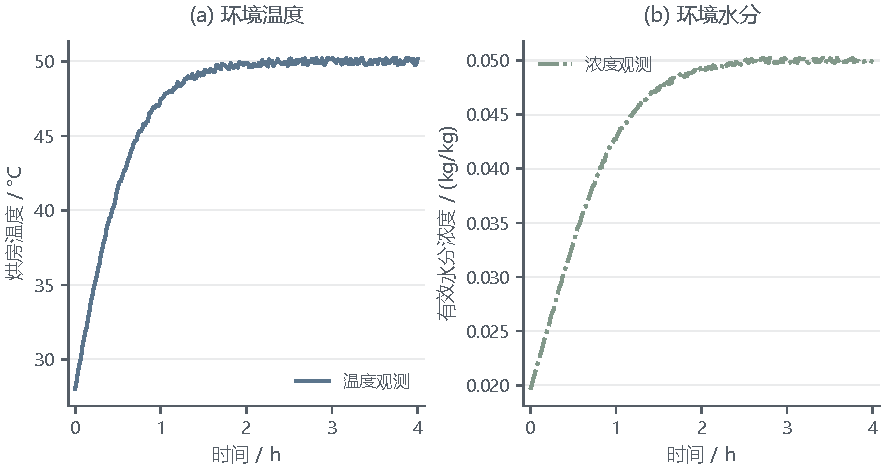
\includegraphics[width=0.86\textwidth,height=5.8cm,keepaspectratio]{figs/raw_q1_environment.pdf}\caption{附件1中烘房温度和有效水分浓度随时间的观测。两个量单位不同，分面展示。}\label{fig:q1-env}\end{figure}
观测时间仅为4小时，远短于两问约51--57小时的报告时长。插值只解决观测窗口内的连续边界读取，窗口以外的末值保持则属于单独的延拓假设。后文的环境覆盖分析将明确指出这一适用边界。

图\ref{fig:q2-env}按观测时间连接环境温度与含湿量，作用是检查输入变化是否同步，不能据此建立温度决定湿度的因果关系，也不能代替药材内部温湿耦合模型。
\begin{figure}[H]\centering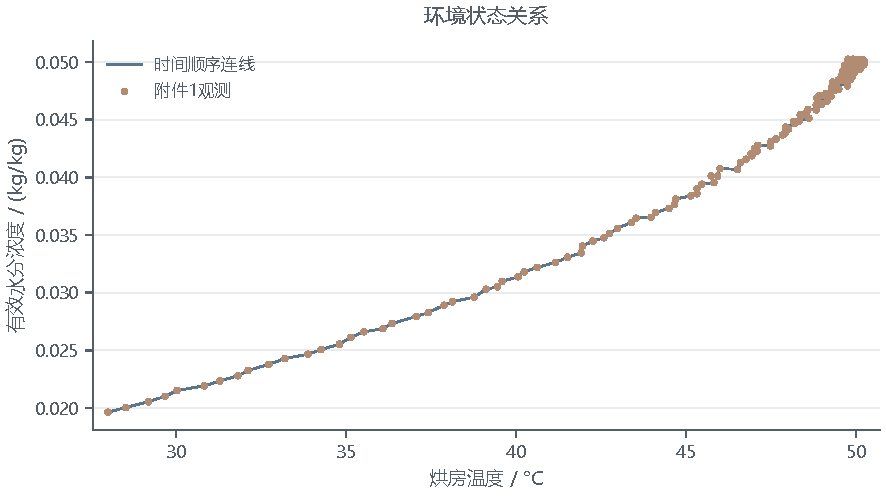
\includegraphics[width=0.86\textwidth,height=5.8cm,keepaspectratio]{figs/raw_q2_environment_relation.pdf}\caption{附件1环境温度与有效水分浓度的关系。曲线按观测时间顺序连接。}\label{fig:q2-env}\end{figure}
\subsection{半径观测及其几何含义}
图\ref{fig:q3-radius}表明收缩主要集中于前期，后期半径逐步接近1.2厘米。相邻观测点间采用线性插值，不人为引入额外收缩参数。该输入决定每个时刻的材料域，因此结果采样必须使用当时的半径，而非一直使用初始2厘米。
\begin{figure}[H]\centering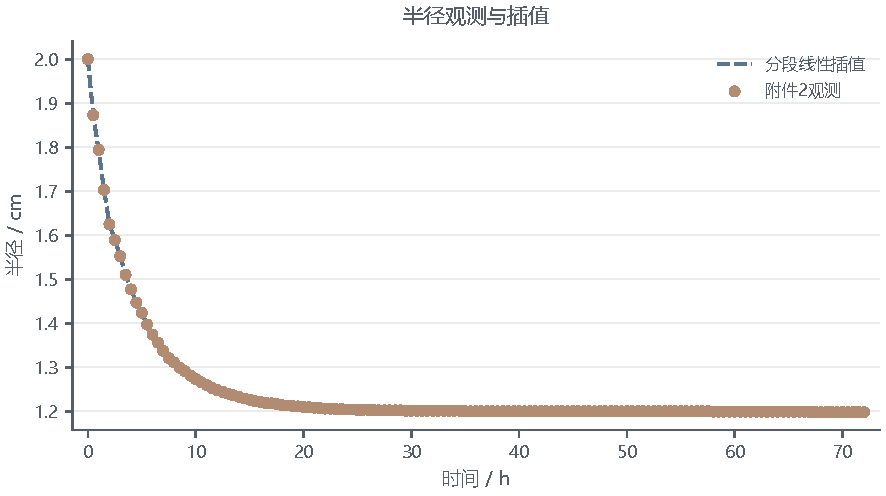
\includegraphics[width=0.86\textwidth,height=5.8cm,keepaspectratio]{figs/raw_q3_radius.pdf}\caption{附件2半径观测及相邻观测点之间的线性插值口径。}\label{fig:q3-radius}\end{figure}
图\ref{fig:q4-radius}以初始半径为基准展示半径比及截面积比。半径缩至初值的约0.6倍时，截面积约为初值的0.36倍；但这不是干物质或水质量的比值，也不能直接换算为干燥时间降幅，因为扩散系数、表面交换和内部状态仍随时间变化。
\begin{figure}[H]\centering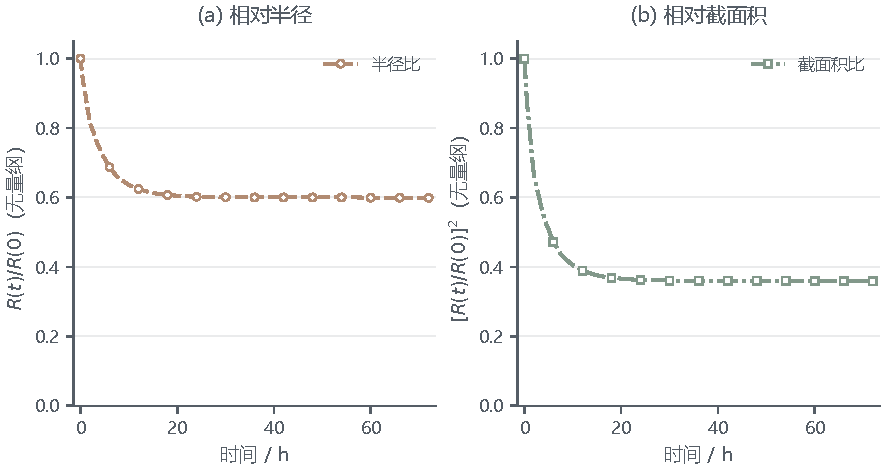
\includegraphics[width=0.86\textwidth,height=5.8cm,keepaspectratio]{figs/raw_q4_shrinkage.pdf}\caption{附件2对应的半径比与截面积比；均为几何量，不表示质量变化。}\label{fig:q4-radius}\end{figure}

\section{统一热湿模型}
在径向等比例材料运动近似下，令$x=r/R(t)\in[0,1]$，$x$为随材料运动的坐标。以下时间导数在固定材料位置取值；这一假设不等同于一般欧拉移动边界问题。温度和含水率控制方程写为
\begin{equation}
\rho(C)c_p(C)\frac{\partial T}{\partial t}\bigg|_x
=\frac{1}{R(t)^2x}\frac{\partial}{\partial x}
\left(xk(C)\frac{\partial T}{\partial x}\right),
\end{equation}
\begin{equation}
\frac{\partial C}{\partial t}\bigg|_x
=\frac{1}{R(t)^2x}\frac{\partial}{\partial x}
\left(xD(C,T_K)\frac{\partial C}{\partial x}\right).
\end{equation}
初值为
\begin{equation}
T(x,0)=28,\qquad C(x,0)=2.55,
\end{equation}
中心边界为
\begin{equation}
\partial_xT(0,t)=0,\qquad\partial_xC(0,t)=0,
\end{equation}
利用题给换热、传质系数构造有效Robin边界：
\begin{equation}
-\frac{k}{R(t)}\partial_xT(1,t)=h(T_s-T_a),\qquad
-\frac{D}{R(t)}\partial_xC(1,t)=h_m(C_s-C_a).
\end{equation}
前三问取$R(t)=R_0$，问题4从附件2在相邻时间点间线性插值获得$R(t)$。

问题1的物性为
\begin{equation}
\rho=820,\quad c_p=2600,\quad k=0.36,\quad D=7\times10^{-9}\exp(-0.89/C).
\end{equation}
问题2、3的物性为
\begin{equation}
\rho=650+128C,\quad c_p=1450+2736\frac{C}{C+1},\quad k=0.21+0.38\frac{C}{C+1},
\end{equation}
\begin{equation}
D=2.4\times10^{-3}\exp\left(-\frac{0.45}{C}-\frac{3850}{T_K}\right).
\end{equation}
问题4的物性为
\begin{equation}
\rho=760+90C,\quad c_p=1850+2150\frac{C}{C+1},\quad k=0.12+0.20\frac{C}{C+1},
\end{equation}
\begin{equation}
D=4.2\times10^{-4}\exp\left(-\frac{0.30}{C}-\frac{3850}{T_K}\right).
\end{equation}

\section{数值方法与改进}
\subsection{区间积分界面通量}
附录3和附录4的扩散系数在低含水率区呈强非线性。对相邻节点$i,i+1$，在面温度$T_{f,i+1/2}=(T_i+T_{i+1})/2$冻结时使用
\begin{equation}
D_{i+1/2}=\int_0^1D((1-s)C_i+sC_{i+1},T_{f,i+1/2})\dd s.
\end{equation}
由8点Gauss--Legendre求积近似。它等价于局部等温单元内对$D(C)$的积分平均，等浓度时自然退化为原扩散系数。非线性热传导中已有将变量相关系数通过积分变换处理的研究\cite{stevens2010}。这里的浓度区间平均由相邻节点之间的局部等温通量积分推得，不是对该文网格自由方法的直接应用，也不将其表述为新的数学变换。

\subsection{表面加密圆环有限体积}
将径向区间分为$N$段，在$N+1$个节点周围建立控制体；节点采用
\begin{equation}
x_i=1-\left(1-\frac{i}{N}\right)^p,\qquad p=2,
\end{equation}
使表面低含水率层获得更小的网格间距。面坐标取$x_{i+1/2}=(x_i+x_{i+1})/2$，控制体权重为
\begin{equation}
V_i=\frac{x_{i+1/2}^2-x_{i-1/2}^2}{2},\quad x_{-1/2}=0,\quad x_{N+1/2}=1.
\end{equation}
对温度或含水率$U$，圆环守恒式为
\begin{equation}
b_iV_i D_t U_i^{n+1}=F_{i+1/2}^{n+1}-F_{i-1/2}^{n+1},
\end{equation}
其中$\Delta x_i=x_{i+1}-x_i$，
\begin{equation}
F_{i+1/2}=\frac{x_{i+1/2}a_{i+1/2}}{R(t_{n+1})^2\Delta x_i}(U_{i+1}^{n+1}-U_i^{n+1}).
\end{equation}
温度取$b_i=\rho_ic_{p,i}$和$a_{i+1/2}=(k_i+k_{i+1})/2$；含水率取$b_i=1$和区间积分的$D_{i+1/2}$。表面外侧PDE通量分别为$-h(T_s-T_a)/R(t)$和$-h_m(C_s-C_a)/R(t)$。

\subsection{非线性时间推进与终点}
第一步使用隐式Euler；有前两次状态后采用变步长BDF2。令$\lambda=h_n/h_{n-1}$，则
\begin{equation}
D_tU=\frac{(1+2\lambda)U^{n+1}-(1+\lambda)^2U^n+\lambda^2U^{n-1}}{h_n(1+\lambda)}.
\end{equation}
每步通过Picard迭代更新物性和状态，状态变化与候选状态方程残差同时验收。残差阈值按代码固定的单位制比较，不是统一的无量纲物理误差界。步长控制比较整步与两半步结果；主算例使用无量纲步长容差$\eta=10^{-4}$。若出现非有限值、$C\le0$、径向单调性违背超过$10^{-10}\max(1,M)$、迭代失败或步长误差超限，则缩短步长；必要时回退隐式Euler，不对负值做裁剪。

定义未达标截面积比例
\begin{equation}
f_{\mathrm{wet}}(t)=2\int_0^1\mathbf 1_{\{C(x,t)\ge C_*\}}x\dd x.
\end{equation}
连续过阈时间定义为
\begin{equation}
t_c =\inf\{t:M(t)<C_*\}.
\end{equation}
当$M$连续时，$M(t_c)$通常等于阈值，严格不等式集合未必存在最小元素。数值报告时刻另记为$t_*=t_R$，取满足未舍入$M(t_R)<C_*$的括号右端；它不是连续定义的精确值。先定位阈值跨越宏步，再保存跨越步的两级历史状态，用同一离散方程二分；事件区间宽度控制为$0.02\,\mathrm s$。该宽度仅是事件搜索宽度，不能代替空间、时间和物理假设的不确定性。



\section{结果与分析}
\subsection{问题1：预热阶段}
图\ref{fig:q1-temp}给出了预热阶段的时间响应。外部热量首先通过表面边界进入药材，随后向中心传递；因此表面曲线先于中心上升。两条曲线之间的间距反映的是空间温差，不能仅以表面温度代表整根药材的温度。
\begin{figure}[H]\centering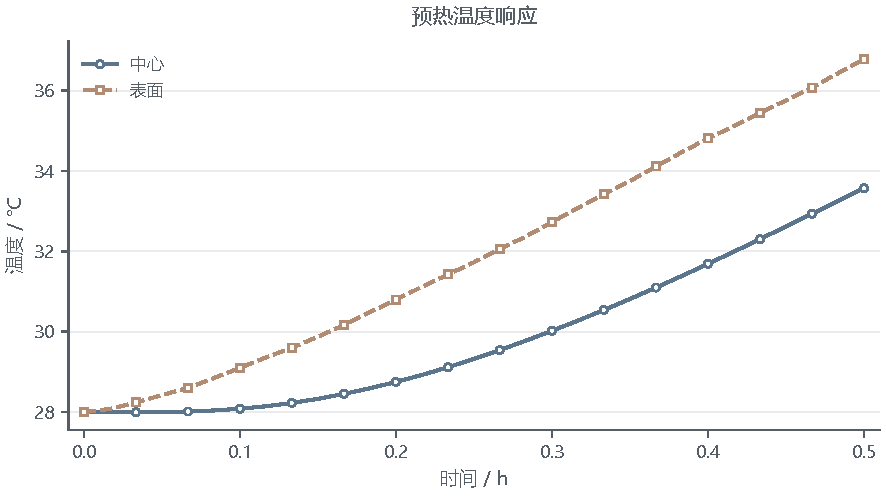
\includegraphics[width=0.86\textwidth,height=5.8cm,keepaspectratio]{figs/process_q1_temperature.pdf}\caption{问题1预热阶段中心和表面温度。表面响应快于中心。}\label{fig:q1-temp}\end{figure}
表\ref{tab:q1t}给出指定位置的温度，表\ref{tab:q1c}给出含水率。图\ref{fig:q1-profile}展示1800秒径向温度剖面。结果显示表面先升温和失水，中心存在明显滞后；在1800秒时中心含水率仍接近初值是方程与边界条件共同作用的结果。

\begin{table}[H]\centering\caption{问题1温度结果（$^{\circ}\mathrm C$）}\label{tab:q1t}\small
\begin{tabular}{rrrrrr}
\toprule 时间/s&0 cm&0.5 cm&1 cm&1.5 cm&2 cm\\\midrule
100&28.0001&28.0004&28.0041&28.0327&28.1801\\
300&28.0408&28.0635&28.1514&28.3681&28.8488\\
600&28.4533&28.5361&28.8040&29.3159&30.1652\\
900&29.3243&29.4583&29.8755&30.6161&31.7304\\
1200&30.5427&30.7098&31.2224&32.1125&33.4276\\
1500&31.9957&32.1868&32.7660&33.7463&35.1203\\
1800&33.5753&33.7721&34.3642&35.3621&36.7856\\
\bottomrule
\end{tabular}\end{table}
\begin{table}[H]\centering\caption{问题1干基含水率结果（kg/kg）}\label{tab:q1c}\small
\begin{tabular}{rrrrrr}
\toprule 时间/s&0 cm&0.5 cm&1 cm&1.5 cm&2 cm\\\midrule
100&2.5500&2.5500&2.5500&2.5500&2.2471\\
300&2.5500&2.5500&2.5500&2.5492&2.0509\\
600&2.5500&2.5500&2.5500&2.5353&1.8770\\
900&2.5500&2.5500&2.5497&2.5045&1.7548\\
1200&2.5500&2.5500&2.5482&2.4646&1.6586\\
1500&2.5500&2.5499&2.5445&2.4206&1.5788\\
1800&2.5500&2.5497&2.5383&2.3755&1.5103\\
\bottomrule
\end{tabular}\end{table}
\begin{figure}[H]\centering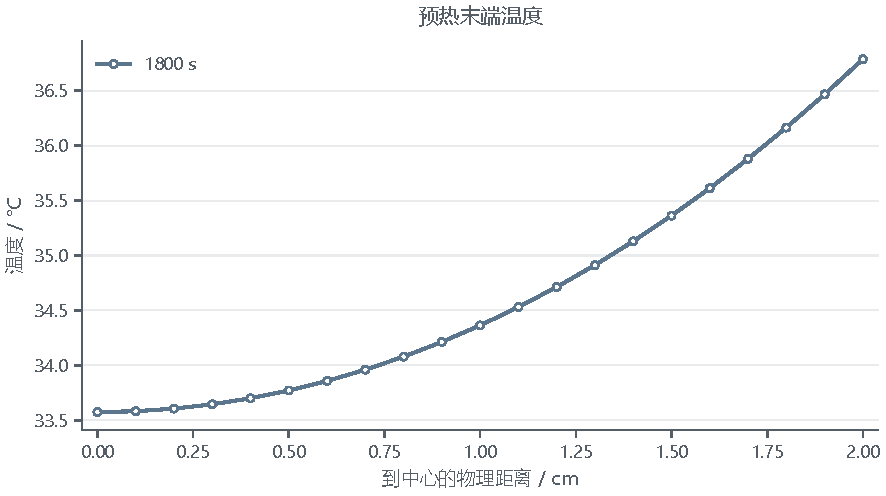
\includegraphics[width=0.86\textwidth,height=5.8cm,keepaspectratio]{figs/result_q1_profile.pdf}\caption{问题1在1800秒的径向温度结果。}\label{fig:q1-profile}\end{figure}
1800秒时，表面与中心温差约3.2103摄氏度，温度随径向位置向外升高；表面含水率约为中心的59.2\%，形成明显的外干内湿分布。短时内中心浓度变化较小不应被视为求解失败，而应结合扩散时间尺度与边界驱动力解释。温度升高与含水率降低不是同一速度的过程。

\subsection{问题2：前3小时与全过程输出}
图\ref{fig:q2-moist}表明失水由快转慢：早期浓度梯度较大，后期表层含水率下降后扩散系数显著降低，内部水分排出受到更强限制。对数纵轴用于同时观察初期高含水率和末期低含水率，不改变原始数值。中心与表面曲线的分离也说明，平均含水率达标不能替代全域达标。
\begin{figure}[H]\centering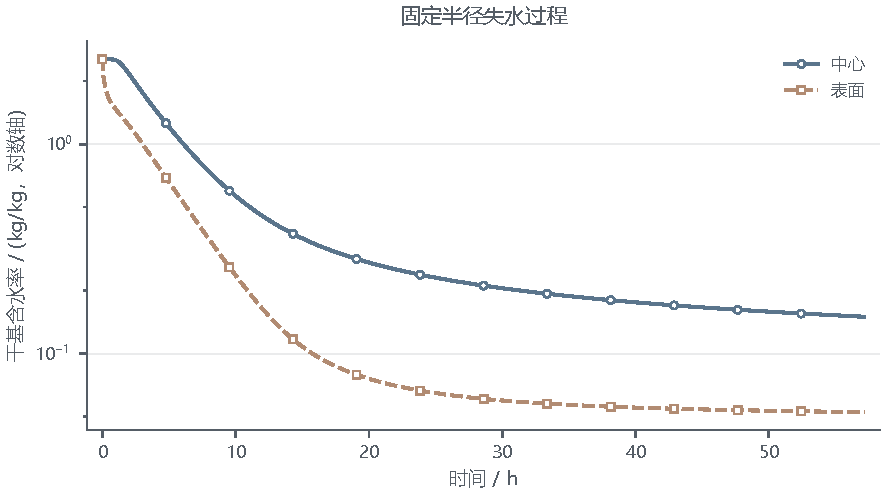
\includegraphics[width=0.86\textwidth,height=5.8cm,keepaspectratio]{figs/process_q2_moisture.pdf}\caption{问题2--3固定半径下中心和表面含水率过程。纵轴采用对数尺度以显示后期低含水率层。}\label{fig:q2-moist}\end{figure}
问题2从初始状态直接使用附录3，不将问题1的1800秒场拼接进来。表\ref{tab:q2t}和表\ref{tab:q2c}给出前3小时结果；完整逐秒矩阵保存在\texttt{改进模型/result2.xlsx}，覆盖$0$到问题3终点，并保留终点事件行。
\begin{table}[H]\centering\caption{问题2前3小时温度结果（$^{\circ}\mathrm C$）}\label{tab:q2t}\small
\begin{tabular}{rrrrrr}\toprule 时间/h&0 cm&0.5 cm&1 cm&1.5 cm&2 cm\\\midrule
0.5&32.1892&32.3822&32.9660&33.9608&35.4130\\
1.0&40.3816&40.5536&41.0605&41.8782&42.9976\\
1.5&45.8468&45.9349&46.1930&46.6051&47.1401\\
2.0&48.4502&48.4881&48.5985&48.7736&49.0033\\
2.5&49.4670&49.4792&49.5137&49.5653&49.6609\\
3.0&49.8495&49.8553&49.8746&49.9101&49.9664\\\bottomrule
\end{tabular}\end{table}
\begin{table}[H]\centering\caption{问题2前3小时干基含水率结果（kg/kg）}\label{tab:q2c}\small
\begin{tabular}{rrrrrr}\toprule 时间/h&0 cm&0.5 cm&1 cm&1.5 cm&2 cm\\\midrule
0.5&2.5499&2.5489&2.5255&2.3257&1.6486\\
1.0&2.5257&2.4947&2.3578&2.0230&1.4711\\
1.5&2.3861&2.3256&2.1344&1.8020&1.3476\\
2.0&2.1709&2.1084&1.9236&1.6259&1.2311\\
2.5&1.9566&1.9006&1.7360&1.4720&1.1166\\
3.0&1.7662&1.7165&1.5702&1.3333&1.0081\\\bottomrule
\end{tabular}\end{table}
\begin{figure}[H]\centering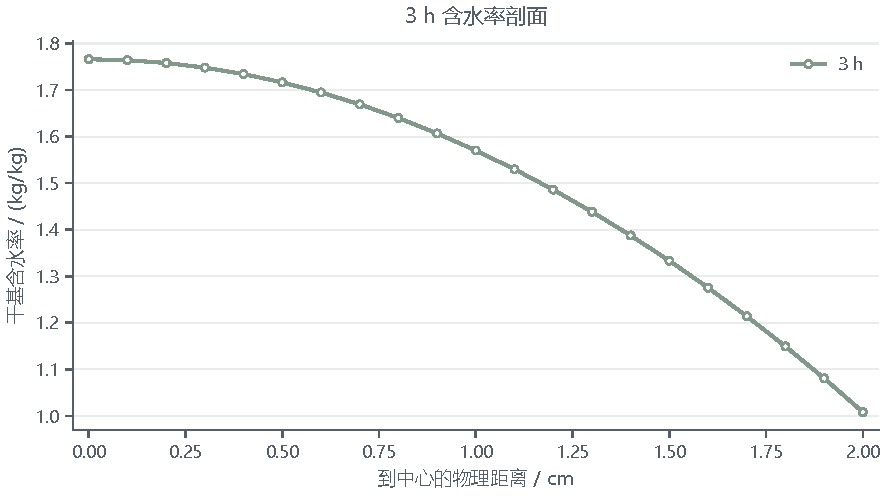
\includegraphics[width=0.86\textwidth,height=5.8cm,keepaspectratio]{figs/result_q2_profile.pdf}\caption{问题2在3小时的径向干基含水率结果。}\label{fig:q2-profile}\end{figure}
图\ref{fig:q2-profile}显示3小时时中心含水率为1.7662千克/千克，表面为1.0081千克/千克，二者均显著高于达标阈值。与此同时，温度已经接近烘房平台值。因此，药材升温接近平衡并不意味着干燥过程完成，后续计算仍需跟踪内部水分向外迁移。

\subsection{问题3：固定半径下的达标时间}
图\ref{fig:q3-wet}将空间场转化为未达标截面积比例。初期即使表面已经失水，大部分内部仍高于阈值；随着干燥推进，未达标区域向中心收缩。该指标便于解释“外干内湿”，但最终结束判据仍采用最大含水率，不能仅以未达标面积在图上看似接近零来停止计算。
\begin{figure}[H]\centering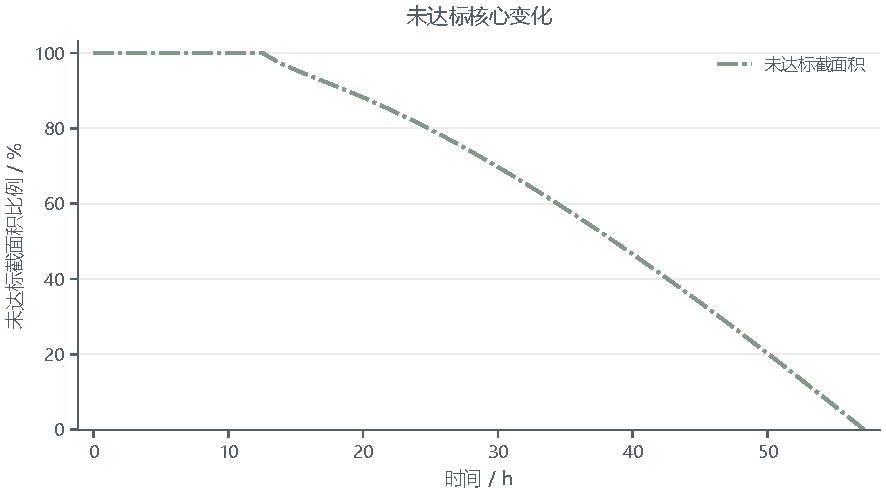
\includegraphics[width=0.86\textwidth,height=5.8cm,keepaspectratio]{figs/process_q3_wet_fraction.pdf}\caption{问题3未达标截面积比例随时间变化。}\label{fig:q3-wet}\end{figure}
问题3与问题2共享附录3物性和固定半径状态轨迹。首次全域达标事件区间为
\[
(205810.51562500,\;205810.53125000]\ \mathrm s,
\]
左端最大含水率为$0.150000001168$，右端最大含水率为$0.149999996588$。因此当前主算例给出
\[
\boxed{t_{*,3}=57.1696\ \mathrm h}.
\]
终点径向剖面如图\ref{fig:q3-end}所示，表\ref{tab:q3}给出每6小时及实际终点的代表性位置结果。
\begin{table}[H]\centering\caption{问题3全过程含水率（kg/kg）}\label{tab:q3}\small
\begin{tabular}{rrrrrr}\toprule 时间/h&0 cm&0.5 cm&1 cm&1.5 cm&2 cm\\\midrule
6&1.0156&0.9868&0.9005&0.7546&0.5335\\
12&0.4548&0.4418&0.4019&0.3289&0.1639\\
18&0.2979&0.2906&0.2679&0.2247&0.0842\\
24&0.2371&0.2321&0.2161&0.1851&0.0663\\
30&0.2053&0.2013&0.1887&0.1637&0.0597\\
36&0.1854&0.1821&0.1714&0.1500&0.0565\\
42&0.1717&0.1687&0.1593&0.1404&0.0547\\
48&0.1615&0.1588&0.1504&0.1332&0.0536\\
54&0.1535&0.1511&0.1433&0.1275&0.0528\\
57.1696&0.1500&0.1477&0.1402&0.1249&0.0525\\\bottomrule
\end{tabular}\end{table}
\begin{figure}[H]\centering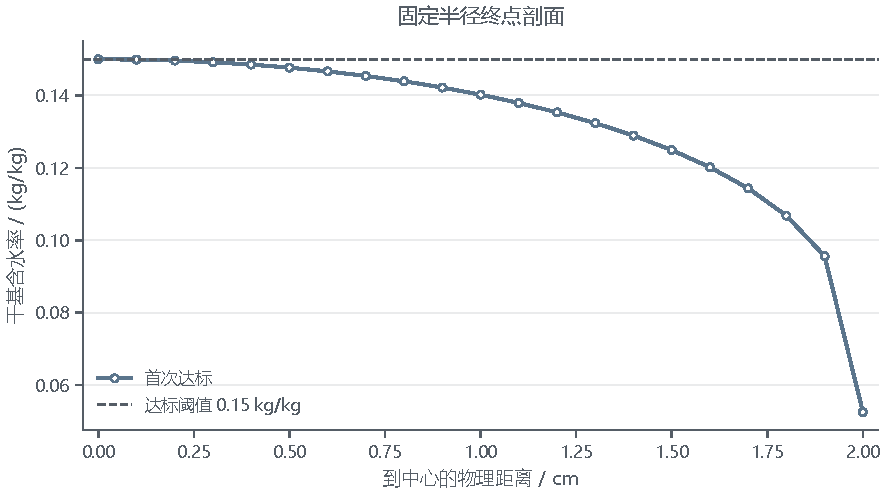
\includegraphics[width=0.86\textwidth,height=5.8cm,keepaspectratio]{figs/result_q3_endpoint.pdf}\caption{问题3首次全域达标时的径向含水率；虚线为$0.15$阈值。}\label{fig:q3-end}\end{figure}
由表\ref{tab:q3}可见，表面在18小时时已低于阈值，而中心仍为0.2979千克/千克；至54小时时中心仍略高于0.15。若仅观察表面，会明显提前结束烘干。终点四舍五入后中心可能显示0.1500，严格判定依据未舍入状态，不能用显示值反推不等式。

\subsection{问题4：考虑收缩与附录4物性}
图\ref{fig:q4-process}分别展示半径和中心含水率。几何收缩使扩散路径变短，同时也改变表面交换项的尺度；两者与状态相关物性共同作用。这里采用共享时间轴的分面，而不使用双纵轴，便于区分厘米与千克/千克两种量纲。
\begin{figure}[H]\centering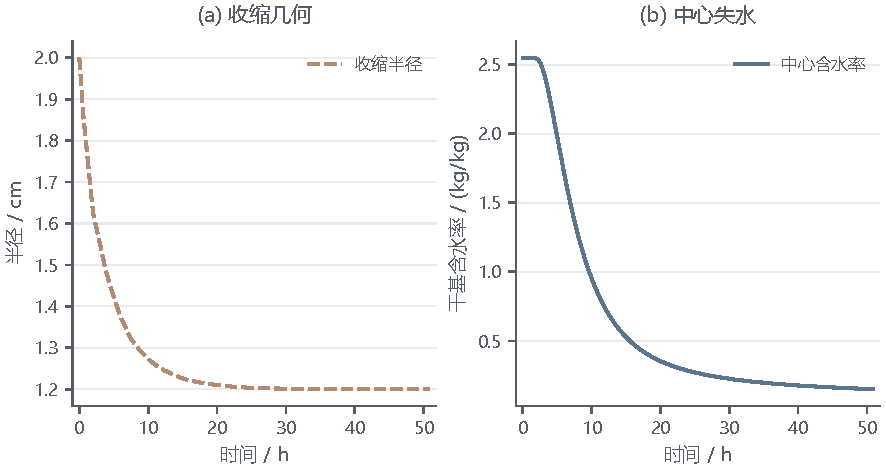
\includegraphics[width=0.86\textwidth,height=5.8cm,keepaspectratio]{figs/process_q4_shrinkage_moisture.pdf}\caption{问题4收缩半径与中心含水率的同步变化，采用分面避免双纵轴造成的比较误导。}\label{fig:q4-process}\end{figure}
问题4使用附件2半径并采用附录4物性。终点事件区间为
\[
(182967.90527344,\;182967.91992188]\ \mathrm s,
\]
左端最大含水率为$0.150000001519$，右端最大含水率为$0.149999993950$。因此当前主算例给出
\[
\boxed{t_{*,4}=50.8244\ \mathrm h},\qquad R(t_{*,4})=1.2000\ \mathrm{cm}.
\]
由于半径不断收缩，固定物理距离$2\,\mathrm{cm}$在6小时后已经超出材料域，因此结果表中该位置留空；“药材表面”列每行取$x=1$节点值。
\begin{table}[H]\centering\caption{问题4全过程含水率（kg/kg）}\label{tab:q4}\small
\begin{tabular}{rrrrrrrr}\toprule 时间/h&0 cm&0.5 cm&1 cm&1.5 cm&2 cm&表面&半径/cm\\\midrule
6&1.7172&1.5357&1.0217&--&--&0.4217&1.3740\\
12&0.7344&0.6518&0.4069&--&--&0.1667&1.2480\\
18&0.4066&0.3668&0.2388&--&--&0.0889&1.2140\\
24&0.2837&0.2599&0.1783&--&--&0.0671&1.2040\\
30&0.2253&0.2085&0.1488&--&--&0.0593&1.2010\\
36&0.1921&0.1790&0.1312&--&--&0.0558&1.2000\\
42&0.1706&0.1598&0.1196&--&--&0.0539&1.2000\\
48&0.1556&0.1463&0.1113&--&--&0.0529&1.2000\\
50.8244&0.1500&0.1413&0.1081&--&--&0.0525&1.2000\\\bottomrule
\end{tabular}\end{table}
表\ref{tab:q4}中的“--”表示对应固定物理距离已超出当前药材域，不表示含水率为零；表面列和半径列记录移动边界上的状态。
\begin{figure}[H]\centering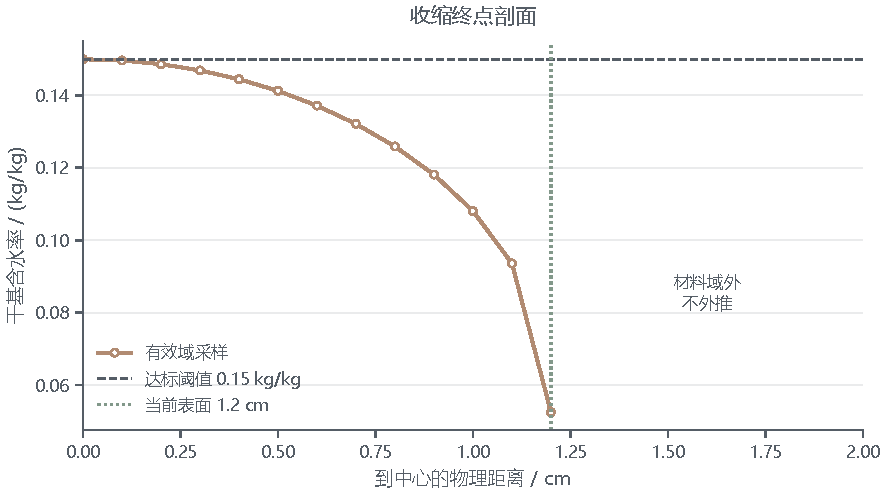
\includegraphics[width=0.86\textwidth,height=5.8cm,keepaspectratio]{figs/result_q4_endpoint.pdf}\caption{问题4首次全域达标时的固定物理距离含水率剖面；有效域外不进行外推。}\label{fig:q4-end}\end{figure}
表\ref{tab:q4}和图\ref{fig:q4-end}使用固定物理距离而不是固定节点编号。6小时时半径约1.3740厘米，所以1.5和2厘米位置不再属于药材；表面位置随时间变化，必须另列。终点的有效域为0--1.2厘米，域外留空有明确几何意义，不应填零或将最外节点强行放到2厘米。

\section{模型检验与敏感性}
\subsection{数值检验}
问题1、2/3、4主算例均保持浓度为正，径向单调性违背量处于浮点舍入量级。表\ref{tab:checks}中的残差来自离散控制体平衡，含水率两列单位为$(\mathrm{kg/kg})/\mathrm s$，不是实测水质量守恒证明。
\begin{table}[H]\centering\caption{主算例数值诊断}\label{tab:checks}\small
\begin{tabular}{lrrrr}\toprule
算例&最低$C$&有效量平衡残差&含水方程残差&拒步次数\\\midrule
问题1&1.51026690&$5.437\times10^{-16}$&$2.044\times10^{-14}$&2\\
问题2/3&0.05253572&$7.923\times10^{-16}$&$6.902\times10^{-14}$&2\\
问题4&0.05249629&$1.701\times10^{-15}$&$5.675\times10^{-14}$&65\\\bottomrule
\end{tabular}\end{table}

数值对照保持161节点、同一边界输入、输出落点和事件规则，将步长误差容差从$10^{-4}$收紧到$10^{-5}$，分别复算问题3和4。另以独立编写的物理圆环矩阵、BDF2推进、整步与两半步误差控制和事件定位程序完成全程对照。独立程序共享题给输入插值及线性代数库，不调用主程序的求解和事件内核；两者一致只能检查实现偏差，不能消除共享物理假设的误差。
\begin{table}[H]\centering\small\caption{容差收紧及独立 BDF2 终点对照}\label{tab:p2}
\begin{tabular}{rrrrr}\toprule 问题&基准/h&收紧容差/h&收紧差/s&独立差/s\\\midrule
3&57.1696&57.1696&+0.0000&+0.0000\\
4&50.8244&50.8244&-0.0146&+0.0000\\
\bottomrule\end{tabular}\end{table}
收紧容差后，问题3终点保持不变，问题4终点变化约$0.0146\,\mathrm s$，低于预先设定的$1\,\mathrm s$终点稳定性验收线。有限空间网格仍存在离散误差，不宣称连续方程真值，未以不同时间配置的混合比较推断空间收敛阶。表\ref{tab:p2}给出容差收紧与独立离散程序的终点对照；详细配置和状态差异见支撑材料中的数值对照数据。

\begin{figure}[H]\centering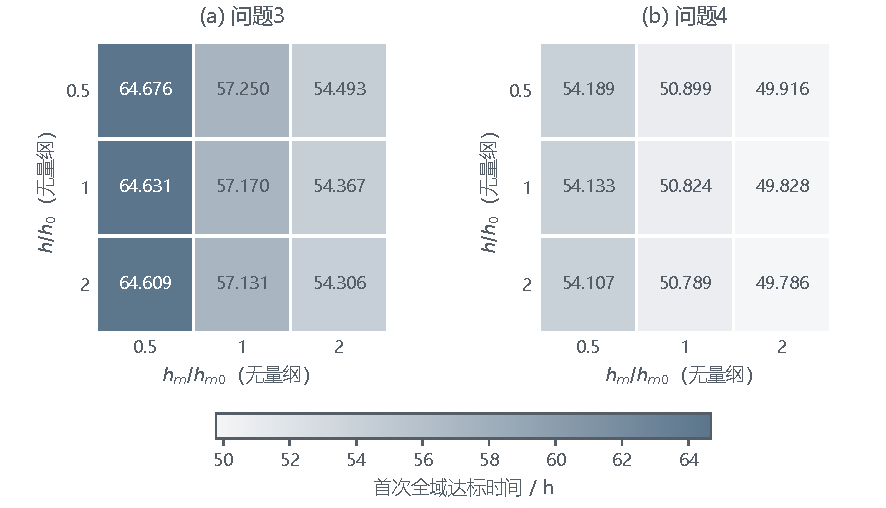
\includegraphics[width=0.96\textwidth,height=6.2cm,keepaspectratio]{figs/p2_boundary_sensitivity.pdf}\caption{换热系数和传质系数的$3\times3$情景扫描。格内为烘干时长（h），所有情景采用同一161节点网格和终点规则。}\label{fig:p2-sensitivity}\end{figure}

\subsection{4小时后环境延拓的证据范围}
附件1止于4小时，主情景在其后保持最后观测值$(T_a,C_a)=(50.165,0.04986)$。题目提到恒温干燥阶段，为温度平台提供定性背景，但不能证明最后一条温度恰为控制设定值，也不能推出空气含湿量始终恒定。问题3有53.1696小时、问题4有46.8244小时位于观测窗口之后，分别占总时长的93.00\%和92.13\%。比例只说明结果对延拓假设的覆盖程度，不是误差比例。

观测最后一小时的61个点等权平均为$(49.9989,0.04998754)$。该均值与末值接近，只反映已观测平台段；它不能证明未来46--53小时仍维持平台。程序虽支持末段均值并以60秒桥接的备选规则，本次没有重新计算该环境情景，故不报告其终点差或宣称环境稳健性通过。若获得后续烘房记录，应先替换延拓再复算问题3、4；当前两问时间均为末值保持条件下的条件性结果。

\subsection{有效浓度边界与热湿闭合}
固体干基含水率的定义是水质量与干物质质量之比；空气的kg/kg可能是水汽与干空气质量之比，题目未进一步给出其基准。两个数的书写单位相同，并不能保证它们是可直接相减的同一热力学变量。较完整的界面模型需要水分活度或吸附等温线，将固体表面含水率与气相湿度联系起来\cite{comsol_sorption,comsol_air}。现式以$C_a$为有效参考量，相当于额外采用恒等映射；$h_m$也应解释为该有效模型中的传递系数，不声称它已完成真实气固界面的标定。

在此单位制下，$-D\partial_r C$的单位是$(\mathrm{kg/kg})\,\mathrm{m/s}$，不能直接当作$\mathrm{kg/(m^2s)}$的蒸发质量通量。引入干物质体积密度并统一质量基准之后，才能构造相应的水质量通量；仅补一个单位换算因子仍不能代替气固相平衡关系。因而，现有边界扫描检验的是有效边界系数变化，不验证其物理闭合。

在真实干燥过程中，汽化引起的能量损失与蒸发质量通量耦合。若相变仅发生于表面、正向$j_{\mathrm{evap}}$表示离开材料的蒸发通量，局部能量关系可写成
\begin{equation}
h(T_a-T_s)=q_{\mathrm{in}}+L_vj_{\mathrm{evap}},
\end{equation}
其中$q_{\mathrm{in}}$为进入材料的导热通量。若相变分布于内部，还需相应体积相变源项；两种表述不能重复计入\cite{comsol_latent}。这里的关系仅说明缺失的闭合，并未加入当前计算模型。比热随含水率变化不自动等价于包含汽化潜热；缺少$j_{\mathrm{evap}}$及其与含水率变化的关系时，也不能直接把有效通量乘潜热当成能量修正。

因此，未计潜热属于未量化的结构误差。蒸发冷却通常会影响表面温度，进而影响温度相关扩散系数，但本题没有完成闭合后的对照计算，不能给出修正时长，更不能把当前时长当成严格上界或下界。数值残差小、两程序一致或名义$h$附近的扫描幅度小，均不能证明潜热影响小。

\subsection{真实干物质与水质量的条件性审查}
令$\rho_d$为单位当前体积中的干物质质量，$\boldsymbol v_s$为固体材料速度，$\boldsymbol j_w$为相对固体的水质量通量。在干物质不流失且没有内部水质量源的理想条件下，需要满足
\begin{equation}
\partial_t\rho_d+\nabla\!\cdot(\rho_d\boldsymbol v_s)=0,\qquad
\partial_t(\rho_d C)+\nabla\!\cdot(\rho_d C\boldsymbol v_s+\boldsymbol j_w)=0.
\end{equation}
结合两式可得$\rho_d\,\mathrm D_sC/\mathrm Dt=-\nabla\!\cdot\boldsymbol j_w$。这里使用材料导数，因此不能仅看到半径变化，就给干基含水率任意补上一个体积稀释项。若另行采用空间均匀且满足$\rho_dR^2L$恒定的干物质密度，并令$\boldsymbol j_w=-\rho_dD\nabla C$，可恢复当前含水率扩散式；但这并不能保证该密度与题给$\rho(C)$一致。

为检验解释的相容性，\textbf{条件性地}将题给$\rho(C)$视为真实湿表观密度，并固定长度$L=0.25\,\mathrm m$。若$C$确为干基含水率，则应有$\rho_d=\rho/(1+C)$，相应积分为
\begin{equation}
m_d(t)=2\pi LR(t)^2\int_0^1\frac{\rho(C)}{1+C}x\dd x,\qquad
m_w(t)=2\pi LR(t)^2\int_0^1\frac{\rho(C)C}{1+C}x\dd x.
\end{equation}
用主情景终点节点和相同圆环权重求积，问题3的$m_d(t_*)/m_d(0)$约为2.1540，问题4约为0.8903，均未维持1。这不是预测药材实际增加或减少了这些干物质，而是说明上述密度、几何和含水率解释不能同时成立。

该判断也有不依赖具体终点剖面的必要条件支持。问题3终点各处$C<0.15$，而$(650+128C)/(1+C)$随$C$下降而增大，在固定体积下干物质比值必大于2.1157；问题4终点$R/R_0=0.6$且$C\ge0$，即使取$C=0$，固定长度下该比值也不超过0.9816。条件性矛盾因此不能由减小时间步消除。

现有程序求解的是有效含水率方程及经验热容量方程；离散平衡量是归一化圆环权重下的含水率积分，不能直接替代真实质量积分。当前缺少独立干物质密度、长度或体积变化、湿质量随时间及真实外排水通量的联合约束，故不使用结果估算实际排水量、能耗或干物质损失率。若补齐这些观测，应重建质量与能量闭合，再重新标定及求解。

\subsection{边界系数扫描的解释与归因范围}
附录3和4没有重复给出$h,h_m$，主算例沿用附录2的$25\,\mathrm{W/(m^2K)}$和$8\times10^{-7}\,\mathrm{m/s}$；各取0.5、1、2倍，共18个全程算例，见图\ref{fig:p2-sensitivity}。这三个倍率是用于压力测试的选点，没有给定概率分布、样本误差模型或置信覆盖率。因此，只能称为确定性参数情景分析。

扫描中问题3的时长范围为54.3055--64.6763小时，问题4为49.7864--54.1887小时。范围只覆盖这9个组合，既不是连续参数域的全局界，也不是统计置信区间。各情景固定了环境延拓、有效边界关系、物性和潜热省略，故没有覆盖这些结构不确定性。

固定$h$为名义值时，$h_m$从0.5倍增至2倍，问题3从64.6309小时降至54.3674小时，问题4从54.1327小时降至49.8283小时。固定$h_m$为名义值、仅改变$h$，两问时间极差约0.1189小时和0.1100小时。只能据此说，在当前有效模型、工况和离散扫描范围内，传质系数扰动对时长的影响更大，不能推广到所有干燥工况。

问题3与问题4的名义时长相差6.3452小时，但两问同时改变了经验物性和几何，差异不能全部归因于收缩。收缩同时改变内部扩散项$R^{-2}$与表面边界项$R^{-1}$；食品干燥研究也说明收缩与结构及工况相关\cite{ramallo2011,mahiuddin2018}。若要区分几何与物性作用，需保持其他条件一致的交叉对照；当前未报告这类归因结果。

\section{模型评价与推广}
\subsection{模型优点}
\textbf{空间判定与题目目标一致。}模型保留径向温湿分布，以全域最大含水率而非平均值确定结束时刻，能够描述表层先干、内部滞后的过程，避免用单点或平均指标替代“各处达标”的要求。

\textbf{四问具有统一的计算框架。}前三问保持固定半径，问题4通过材料坐标引入实测收缩，仅按题意切换物性和几何输入。相同框架便于追溯差异来自哪些条件，也使温湿场与结果表的采样口径保持一致。

\textbf{强非线性处理有针对性。}区间积分面系数避免仅依赖端点扩散系数，表面加密改善干燥外层的空间分辨率；隐式推进与迭代检查相结合，能够处理低含水率阶段较慢的内部迁移。容差收紧和独立实现对照为数值结果提供了实现层面的检验，而非依靠图形光滑判断可靠性。
\subsection{模型缺陷及其影响}
\textbf{环境延拓决定了大部分预测时段。}前4小时以外没有环境记录，问题3、4超过九成的时间位于观测窗口之后。末值保持使计算可复现，但无法反映控温波动、空气含湿量累积及换气制度变化；报告时长应始终附带这一工况条件。

\textbf{气固边界尚未完成物理标定。}空气含湿量与固体干基含水率采用有效恒等映射，缺少吸附等温线或水分活度关系。边界参数扫描只能说明当前有效系数变化带来的结果差，不能验证真实气固界面交换规律。

\textbf{潜热与真实质量闭合缺失。}现有热方程不含蒸发相变项，不能用来可靠估计烘干能耗。条件性质量审查进一步表明，题给密度、既定几何与干基含水率不能同时解释为严格真实质量闭合；因此不能将归一化含水率平衡残差当作真实排水量或干物质守恒证明。

\textbf{几何简化与空间精度仍有限。}一维轴对称和径向等比例收缩忽略了端部、非均匀形变及材料各向异性。即使时间容差收紧后终点稳定，有限空间网格及共享物理假设的误差也不会自动消失。独立程序一致只能排查实现差异，不能替代实测温湿剖面对照。
\subsection{推广条件与改进路径}
模型可作为相近圆柱状材料的有效干燥分析框架，但不能直接迁移本题经验系数。推广至其他药材或食品时，应先获得相应物性、平衡吸附关系及几何变化数据，再重新校准。若长度与端部效应显著，应改为二维轴对称模型；若存在明显非均匀收缩，应以实测形变或力学模型替代等比例材料坐标。

建议优先补测后续环境、总湿质量和体积变化，使边界与质量口径得到约束；随后引入与真实蒸发通量相容的潜热项，再用独立温湿剖面验证参数。完成这些步骤后，才适合进一步讨论温湿工艺优化、能耗与品质约束，而不是在当前数据不足的条件下叠加未经辨识的参数。
\section{结论}
在题给经验物性与末值保持环境条件下，预热阶段存在明显径向温湿滞后；固定半径模型的报告干燥时长为57.1696小时，采用附录4与实测收缩半径后为50.8244小时，终点半径1.2000厘米。两问名义时长差为6.3452小时，不能视为收缩的单独因果效应。

通过容差收紧和独立离散程序对照，报告终点具有所检验条件下的数值稳定性。边界情景结果显示，在离散扫描范围内传质系数对时长的影响较大。上述结论属于明确假设下的有效模型预测；环境延拓、气固平衡、潜热和真实质量闭合仍是后续物理验证的关键。

\bibliographystyle{unsrt}
\bibliography{references}

\clearpage
\appendix
\section{支撑材料文件列表}
支撑材料保留主程序、四份结果表、22份数值对照记录及已有验证记录，并按原目录层级附上题给输入与结果模板。较大的主轨迹缓存不随精简包分发，可按README重建。结果状态保留四位小数，实际终点采用未舍入状态判定；已有验证记录不代表本次再次运行。
\begin{longtable}{>{\raggedright\arraybackslash}p{.45\textwidth}>{\raggedright\arraybackslash}p{.47\textwidth}}
\caption{支撑材料文件及用途}\label{tab:support-files}\\
\toprule 文件或目录&内容\\\midrule
\texttt{README.md}\newline\texttt{reproduce.py}&环境、目录说明与统一复现入口\\
\texttt{改进模型/result1.xlsx}\newline\texttt{改进模型/result2.xlsx}&温度与水分浓度，每1秒、0.1厘米\\
\texttt{改进模型/result3.xlsx}\newline\texttt{改进模型/result4.xlsx}&水分浓度，每60秒、0.1厘米；问题4另有表面及半径\\
\texttt{改进模型/*.py}&主求解、输出、绘图、独立参考与验证源码\\
\texttt{改进模型/requirements*.txt}&依赖范围及原运行环境的锁定版本\\
\texttt{改进模型/p2/runs/*.json}&22个数值对照算例的配置、终点和状态\\
\texttt{改进模型/verification.json}&续接工作区已有Excel回读记录；复算时更新\\
\texttt{科学假设诊断.json}&条件性密度质量与环境覆盖诊断\\
\texttt{附件/附件1.xlsx}\newline\texttt{附件/附件2.xlsx}\newline\texttt{附件/附件3/result*.xlsx}&原题环境、收缩数据及四份空结果模板\\
\texttt{验证/}&已有Excel与P2汇总的留存件，以及六条引用核对来源\\
\texttt{文件来源.json}\newline\texttt{SHA256SUMS.txt}&逐文件来源与整理时的字节指纹清单\\
\bottomrule
\end{longtable}
表\ref{tab:support-files}列出与模型计算和结果输出对应的支撑文件。

\section{完整源程序}
运行环境为Python 3.12、NumPy、SciPy、openpyxl和Matplotlib；安装版本与命令见支撑材料README。原始输入使用题目附件1、2，放置在源程序上一级的“附件”目录。下列源码与支撑材料一致。
\subsection{build\_outputs.py}
\begin{verbatim}
"""Portable result reproduction from the frozen canonical trajectories.
Only four-decimal exports; no invented version-comparison tables.
"""
import gzip
import json
import shutil
from pathlib import Path
import numpy as np
from openpyxl import Workbook
from openpyxl.cell import WriteOnlyCell
from openpyxl.utils import get_column_letter
from model import sample

ROOT=Path(__file__).resolve().parent

def write_book(name,sheets):
    wb=Workbook(write_only=True)
    for title,states,field,moving in sheets:
        ws=wb.create_sheet(title)
        ws.freeze_panes='B2';ws.column_dimensions['A'].width=25
        for j in range(2,25):ws.column_dimensions[get_column_letter(j)].width=12
        header=['时间/s；距离/cm']+[round(x/10,1) for x in range(21)]
        if moving:header+=['药材表面','表面半径/cm']
        ws.append(header)
        for state in states:
            vals=sample(state,field,np.arange(21)/10)
            if moving:vals+=[state[field][-1],state['radius_cm']]
            values=[state['t']]+[None if v is None else round(v,4) for v in vals]
            cells=[WriteOnlyCell(ws,value=v) for v in values]
            for c in cells:c.number_format='0.0000'
            ws.append(cells)
    path=ROOT/name
    wb.save(path)
    (ROOT/'results').mkdir(exist_ok=True)
    shutil.copy2(path,ROOT/'results'/name)

def main():
    for name,number in [('q1_final',1),('q2_full',2),('q4_final',4)]:
        with gzip.open(ROOT/'runs'/f'{name}.json.gz','rt',encoding='utf-8') as f:
            result=json.load(f)
        if number in (1,2):
            write_book(f'result{number}.xlsx',[(title,result['short'],field,False)
                for title,field in [('温度','T'),('水分浓度','C')]])
            if number==2:write_book('result3.xlsx',[('Sheet1',result['long'],'C',False)])
        else:write_book('result4.xlsx',[('Sheet1',result['long'],'C',True)])
        print('exported',name,flush=True)
        del result

if __name__=='__main__':main()

\end{verbatim}

\subsection{make\_figures.py}
\begin{verbatim}
"""Generate v0.4 publication figures from frozen run caches."""
from pathlib import Path
import gzip, json, sys
import numpy as np

import matplotlib
matplotlib.use('Agg')
import matplotlib.pyplot as plt

import shutil

from model import ROOT, sample


def load(name):
    with gzip.open(ROOT / 'runs' / f'{name}.json.gz', 'rt', encoding='utf8') as f:
        return json.load(f)


def save(fig, stem):
    for extension in ('pdf','svg','png'):
        path=ROOT/'figures'/f'{stem}.{extension}'
        fig.savefig(path,dpi=180,bbox_inches='tight')
        if extension=='pdf':
            target=ROOT.parent/'完整论文-LaTeX/figs'
            target.mkdir(parents=True,exist_ok=True)
            shutil.copy2(path,target/path.name)
    plt.close(fig)


def main():
    plt.rcParams.update({'font.family':['DejaVu Serif','SimSun'],
        'font.size':11,'axes.unicode_minus':False,'mathtext.fontset':'dejavuserif',
        'pdf.fonttype':42,'svg.fonttype':'path'})
    q1, q2, q4 = load('q1_final'), load('q2_full'), load('q4_final')
    q3 = q2
    figdir = ROOT / 'figures'
    figdir.mkdir(exist_ok=True)
    colors = ['#0072B2', '#D55E00', '#009E73', '#CC79A7']
    # Raw data figures: observed environmental and radius data, plus derived ranges.
    # q1: two observed air variables, separate panels because units differ.
    from model import Inputs
    inp = Inputs()
    fig, ax = plt.subplots(1, 2, figsize=(7.2, 4.2), constrained_layout=True)
    ax[0].plot(inp.air[:, 0] / 3600, inp.air[:, 1], color=colors[0])
    ax[0].set(xlabel='时间 / h', ylabel='烘房温度 / °C', title='附件1：烘房温度')
    ax[1].plot(inp.air[:, 0] / 3600, inp.air[:, 2], color=colors[2])
    ax[1].set(xlabel='时间 / h', ylabel='有效水分浓度 / (kg/kg)', title='附件1：烘房水分浓度')
    for a in ax: a.spines[['top', 'right']].set_visible(False)
    save(fig, 'raw_q1_environment')
    # q2: input range summary as a relationship between environment variables.
    fig, ax = plt.subplots(figsize=(7.2, 4.2), constrained_layout=True)
    ax.plot(inp.air[:, 1], inp.air[:, 2], color=colors[0], lw=1.0, marker='o', ms=1.5)
    ax.set(xlabel='烘房温度 / °C', ylabel='烘房水分浓度 / (kg/kg)', title='附件1：环境状态关系')
    ax.spines[['top', 'right']].set_visible(False)
    save(fig, 'raw_q2_environment_relation')
    # q3: radius-independent observed data context.
    fig, ax = plt.subplots(figsize=(7.2, 4.2), constrained_layout=True)
    ax.scatter(inp.radii[:, 0] / 3600, inp.radii[:, 1], s=12, color=colors[1], label='观测')
    ax.plot(inp.radii[:, 0] / 3600, inp.radii[:, 1], color=colors[1], alpha=.6)
    ax.set(xlabel='时间 / h', ylabel='半径 / cm', title='附件2：药材半径观测与线性插值')
    ax.legend(frameon=False); ax.spines[['top', 'right']].set_visible(False)
    save(fig, 'raw_q3_radius')
    # q4 raw: combined normalized radius and environmental temperature.
    fig, ax = plt.subplots(figsize=(7.2, 4.2), constrained_layout=True)
    ax.plot(inp.radii[:, 0] / 3600, inp.radii[:, 1] / inp.radii[0, 1], color=colors[1])
    ax.set(xlabel='时间 / h', ylabel='R(t) / R(0)', title='收缩几何的无量纲半径')
    ax.spines[['top', 'right']].set_visible(False)
    save(fig, 'raw_q4_shrinkage')

    # Process figures.
    s1 = q1['long']
    fig, ax = plt.subplots(figsize=(7.2, 4.2), constrained_layout=True)
    tt = np.array([s['t'] for s in s1]) / 3600
    ax.plot(tt, [s['T'][0] for s in s1], color=colors[0], label='中心')
    ax.plot(tt, [s['T'][-1] for s in s1], color=colors[1], label='表面')
    ax.set(xlabel='时间 / h', ylabel='温度 / °C', title='问题1：预热阶段中心—表面温度')
    ax.legend(frameon=False); ax.spines[['top', 'right']].set_visible(False)
    save(fig, 'process_q1_temperature')
    fig, ax = plt.subplots(figsize=(7.2, 4.2), constrained_layout=True)
    ss = q2['long']; tt = np.array([s['t'] for s in ss]) / 3600
    ax.plot(tt, [s['C'][0] for s in ss], color=colors[0], label='中心')
    ax.plot(tt, [s['C'][-1] for s in ss], color=colors[1], label='表面')
    ax.set(xlabel='时间 / h', ylabel='干基含水率 / (kg/kg)', title='问题2—3：固定半径失水过程')
    ax.set_yscale('log'); ax.legend(frameon=False); ax.spines[['top', 'right']].set_visible(False)
    save(fig, 'process_q2_moisture')
    fig, ax = plt.subplots(figsize=(7.2, 4.2), constrained_layout=True)
    ax.plot(tt, [100*s['wet_fraction'] for s in ss], color=colors[2])
    ax.axhline(0, color='#555', lw=.8)
    ax.set(xlabel='时间 / h', ylabel='未达标截面积比例 / %', title='问题3：未达标核心面积变化')
    ax.spines[['top', 'right']].set_visible(False)
    save(fig, 'process_q3_wet_fraction')
    ss4 = q4['long']; tt4 = np.array([s['t'] for s in ss4]) / 3600
    fig, ax = plt.subplots(1, 2, figsize=(7.2, 4.2), constrained_layout=True)
    ax[0].plot(tt4, [s['radius_cm'] for s in ss4], color=colors[1])
    ax[0].set(xlabel='时间 / h', ylabel='半径 / cm', title='收缩半径')
    ax[1].plot(tt4, [s['C'][0] for s in ss4], color=colors[0])
    ax[1].set(xlabel='时间 / h', ylabel='中心含水率 / (kg/kg)', title='中心含水率')
    for a in ax: a.spines[['top', 'right']].set_visible(False)
    save(fig, 'process_q4_shrinkage_moisture')

    # Result figures: spatial fields and endpoint profiles.
    dist = np.arange(0, 2.001, .1)
    snap1 = q1['summaries']['1800']; valsT = sample(snap1, 'T', dist); valsC = sample(snap1, 'C', dist)
    fig, ax = plt.subplots(figsize=(7.2, 4.2), constrained_layout=True)
    ax.plot(dist, valsT, color=colors[0], label='温度')
    ax.set(xlabel='到中心距离 / cm', ylabel='温度 / °C', title='问题1：1800 s径向温度结果')
    ax.spines[['top', 'right']].set_visible(False)
    save(fig, 'result_q1_profile')
    snap2 = q2['summaries']['10800']; vals = sample(snap2, 'C', dist)
    fig, ax = plt.subplots(figsize=(7.2, 4.2), constrained_layout=True)
    ax.plot(dist, vals, color=colors[2], marker='o', ms=2, label='3 h')
    ax.set(xlabel='到中心距离 / cm', ylabel='干基含水率 / (kg/kg)', title='问题2：3 h径向含水率结果')
    ax.spines[['top', 'right']].set_visible(False)
    save(fig, 'result_q2_profile')
    vals = sample(q2['final'], 'C', dist)
    fig, ax = plt.subplots(figsize=(7.2, 4.2), constrained_layout=True)
    ax.plot(dist, vals, color=colors[0], marker='o', ms=2)
    ax.axhline(.15, color='#555', ls='--', label='阈值 0.15')
    ax.set(xlabel='到中心距离 / cm', ylabel='干基含水率 / (kg/kg)', title='问题3：首次达标时径向含水率')
    ax.legend(frameon=False); ax.spines[['top', 'right']].set_visible(False)
    save(fig, 'result_q3_endpoint')
    vals = sample(q4['final'], 'C', dist)
    fig, ax = plt.subplots(figsize=(7.2, 4.2), constrained_layout=True)
    ax.plot(dist, vals, color=colors[1], marker='o', ms=2, label='有效域采样')
    ax.axhline(.15, color='#555', ls='--', label='阈值 0.15')
    ax.set(xlabel='固定物理距离 / cm', ylabel='干基含水率 / (kg/kg)', title='问题4：收缩终点物理距离剖面')
    ax.legend(frameon=False); ax.spines[['top', 'right']].set_visible(False)
    save(fig, 'result_q4_endpoint')
    print('figures generated: 12 logical figures')
if __name__ == '__main__':
    main()

\end{verbatim}

\subsection{model.py}
\begin{verbatim}
"""Versioned nonlinear radial heat/moisture solver for 2026 CUMCM A.

v0.4: nonuniform surface-graded finite volumes, variable-step BDF2 with
implicit-Euler fallback, exact output-grid landing, and endpoint guards.
The physical interpretation remains the题设 effective heat/moisture model;
this implementation does not add latent-heat or dry-matter closure terms.
"""
from dataclasses import dataclass, asdict
from functools import lru_cache
from pathlib import Path
import time
import numpy as np
import openpyxl
from scipy.linalg import solve_banded

ROOT = Path(__file__).resolve().parent

@lru_cache(maxsize=None)
def gauss(order):
    z, w = np.polynomial.legendre.leggauss(order)
    return (z + 1.0) / 2.0, w / 2.0


def properties(material, c, t):
    c = np.asarray(c, dtype=float)
    t = np.asarray(t, dtype=float)
    if material == 1:
        return (np.full_like(c, 820.0 * 2600.0), np.full_like(c, 0.36),
                7e-9 * np.exp(-0.89 / c))
    if material == 3:
        return ((650.0 + 128.0 * c) * (1450.0 + 2736.0 * c / (c + 1.0)),
                0.21 + 0.38 * c / (c + 1.0),
                2.4e-3 * np.exp(-0.45 / c - 3850.0 / (t + 273.15)))
    if material == 4:
        return ((760.0 + 90.0 * c) * (1850.0 + 2150.0 * c / (c + 1.0)),
                0.12 + 0.20 * c / (c + 1.0),
                4.2e-4 * np.exp(-0.30 / c - 3850.0 / (t + 273.15)))
    raise ValueError(material)


def integral_diffusivity(material, left, right, tface, order=8):
    left = np.asarray(left, dtype=float)
    right = np.asarray(right, dtype=float)
    tface = np.asarray(tface, dtype=float)
    z, w = gauss(order)
    c = left[:, None] + (right - left)[:, None] * z
    if material == 1:
        vals = 7e-9 * np.exp(-0.89 / c)
    elif material == 3:
        vals = 2.4e-3 * np.exp(-0.45 / c - 3850.0 / (tface[:, None] + 273.15))
    elif material == 4:
        vals = 4.2e-4 * np.exp(-0.30 / c - 3850.0 / (tface[:, None] + 273.15))
    else:
        raise ValueError(material)
    return vals @ w


@dataclass
class Config:
    material: int = 3
    shrink: bool = False
    n: int = 80
    grid_power: float = 2.0
    early_dt: float = 1.0
    late_dt: float = 15.0
    quadrature: int = 8
    method: str = 'bdf2'
    tolerance: float = 1e-9
    residual_tolerance: float = 2e-8
    step_tolerance: float = 1e-4
    max_iterations: int = 40
    endpoint_tolerance: float = 0.02
    min_dt: float = 0.01
    max_retries: int = 8
    max_time: float = 7 * 86400.0
    stop_dry: bool = True
    keep_short: bool = False
    compact_output: bool = False
    output_stride: int = 60
    environment: str = 'last'


class Inputs:
    def __init__(self):
        data = []
        for name in ('附件1.xlsx', '附件2.xlsx'):
            path = ROOT.parent / '附件' / name
            wb = openpyxl.load_workbook(path, data_only=True, read_only=True)
            rows = list(wb.active.values)
            wb.close()
            a = np.asarray(rows[1:], dtype=float)
            if not np.isfinite(a).all() or not np.all(np.diff(a[:, 0]) > 0):
                raise ValueError(f'invalid input: {name}')
            data.append(a)
        self.air, self.radii = data

    def boundary(self, t, environment='last'):
        a = self.air
        if t > a[-1, 0] and environment == 'last_hour_mean':
            block = a[a[:, 0] >= a[-1, 0] - 3600.0, 1:]
            target = block.mean(axis=0)
            if t <= a[-1, 0] + 60.0:
                w = (t - a[-1, 0]) / 60.0
                return tuple((1.0 - w) * a[-1, 1:] + w * target)
            return tuple(target)
        return (float(np.interp(t, a[:, 0], a[:, 1])),
                float(np.interp(t, a[:, 0], a[:, 2])))

    def radius(self, t, shrink):
        if not shrink:
            return 0.02
        if t > self.radii[-1, 0] + 1e-8:
            raise ValueError('Shrinkage data extrapolation is not allowed')
        return 0.01 * float(np.interp(t, self.radii[:, 0], self.radii[:, 1]))


class StepFailure(RuntimeError):
    pass


class Solver:
    def __init__(self, config, inputs=None):
        cfg = config
        if cfg.n < 2 or cfg.grid_power < 1:
            raise ValueError('invalid grid')
        if cfg.keep_short and cfg.output_stride < 1:
            raise ValueError('output_stride must be positive')
        self.cfg = cfg
        self.inputs = inputs or Inputs()
        self.x = 1.0 - (1.0 - np.arange(cfg.n + 1, dtype=float) / cfg.n) ** cfg.grid_power
        self.face = (self.x[:-1] + self.x[1:]) / 2.0
        self.edges = np.r_[0.0, self.face, 1.0]
        self.volume = np.diff(self.edges ** 2) / 2.0
        self.dx = np.diff(self.x)
        self.output_distances_cm = np.arange(0.0, 2.001, 0.1)
        self.stats = {
            'steps': 0, 'iterations': 0, 'rejected_steps': 0,
            'max_iterations': 0, 'max_mass_balance_residual': 0.0,
            'max_moisture_equation_residual': 0.0,
            'max_heat_equation_residual': 0.0,
            'bdf2_steps': 0, 'euler_steps': 0, 'event_fallbacks': 0,
            'step_failures': 0, 'max_step_error': 0.0,
        }

    def coefficients(self, face_coefficient, capacity, boundary, radius, dt):
        face_coefficient = np.asarray(face_coefficient, dtype=float)
        capacity = np.asarray(capacity, dtype=float)
        g = self.face * face_coefficient / (self.dx * radius ** 2)
        left = dt * np.r_[0.0, g] / (self.volume * capacity)
        right = dt * np.r_[g, 0.0] / (self.volume * capacity)
        conv = dt * boundary / (radius * self.volume[-1] * capacity[-1])
        ab = np.zeros((3, len(capacity)), dtype=float)
        ab[0, 1:] = -right[:-1]
        ab[1, :] = 1.0 + left + right
        ab[1, -1] += conv
        ab[2, :-1] = -left[1:]
        return ab, conv

    def linear_step(self, u, face_coefficient, capacity, boundary, ambient, radius, dt):
        ab, conv = self.coefficients(face_coefficient, capacity, boundary, radius, dt)
        rhs = np.asarray(u, dtype=float).copy()
        rhs[-1] += conv * ambient
        return solve_banded((1, 1), ab, rhs, check_finite=False)

    def _bdf_coefficients(self, dt, previous_dt, has_history, method=None):
        method = method or self.cfg.method
        if method != 'bdf2' or not has_history or previous_dt is None:
            return 1.0 / dt, -1.0 / dt, 0.0, 'euler'
        ratio = dt / previous_dt
        if ratio < 0.5 - 1e-12 or ratio > 2.0 + 1e-12:
            return 1.0 / dt, -1.0 / dt, 0.0, 'euler'
        return ((1.0 + 2.0 * ratio) / (dt * (1.0 + ratio)),
                -(1.0 + ratio) ** 2 / (dt * (1.0 + ratio)),
                ratio ** 2 / (dt * (1.0 + ratio)), 'bdf2')

    def _linear_general(self, old, previous, face_coefficient, capacity,
                        boundary, ambient, radius, dt, a0, a1, a2):
        capacity = np.asarray(capacity, dtype=float)
        g = self.face * np.asarray(face_coefficient, dtype=float) / (self.dx * radius ** 2)
        scale = 1.0 / a0
        left = scale * np.r_[0.0, g] / (self.volume * capacity)
        right = scale * np.r_[g, 0.0] / (self.volume * capacity)
        conv = scale * boundary / (radius * self.volume[-1] * capacity[-1])
        ab = np.zeros((3, len(capacity)), dtype=float)
        ab[0, 1:] = -right[:-1]
        ab[1, :] = 1.0 + left + right
        ab[1, -1] += conv
        ab[2, :-1] = -left[1:]
        history_rhs = -(a1 * old + a2 * previous) / a0
        history_rhs = np.asarray(history_rhs, dtype=float)
        history_rhs[-1] += conv * ambient
        return solve_banded((1, 1), ab, history_rhs, check_finite=False)

    def _residual(self, old, previous, new, face_coefficient, capacity,
                  boundary, ambient, radius, dt, a0, a1, a2):
        capacity = np.asarray(capacity, dtype=float)
        g = self.face * np.asarray(face_coefficient, dtype=float) / (self.dx * radius ** 2)
        flux_left = np.r_[0.0, g] * (new - np.r_[new[0], new[:-1]])
        flux_right = np.r_[g, 0.0] * (np.r_[new[1:], new[-1]] - new)
        flux_right[-1] = -boundary * (new[-1] - ambient) / radius
        # equation is capacity*V*Dt - (F_right-F_left)=0
        lhs = capacity * self.volume * (a0 * new + a1 * old + a2 * previous)
        return lhs - (flux_right - flux_left)

    def diffusion_faces(self, c, temp):
        if self.cfg.method == 'arithmetic':
            d = properties(self.cfg.material, c, temp)[2]
            return (d[:-1] + d[1:]) / 2.0
        return integral_diffusivity(
            self.cfg.material, c[:-1], c[1:],
            (temp[:-1] + temp[1:]) / 2.0, self.cfg.quadrature)

    def _attempt(self, t, old_t, old_c, prev_t, prev_c, previous_dt, dt, force_method=None):
        cfg = self.cfg
        ta, ca = self.inputs.boundary(t + dt, cfg.environment)
        radius = self.inputs.radius(t + dt, cfg.shrink)
        has_history = prev_t is not None and prev_c is not None and previous_dt is not None
        a0, a1, a2, actual_method = self._bdf_coefficients(
            dt, previous_dt, has_history, force_method)
        previous_t = old_t if prev_t is None else prev_t
        previous_c = old_c if prev_c is None else prev_c
        new_t = old_t.copy()
        new_c = old_c.copy()
        previous_error = np.inf
        damping = 1.0
        last = None
        for it in range(1, cfg.max_iterations + 1):
            cap, k, _ = properties(cfg.material, new_c, new_t)
            ts = self._linear_general(
                old_t, previous_t, (k[:-1] + k[1:]) / 2.0, cap,
                25.0, ta, radius, dt, a0, a1, a2)
            dface = self.diffusion_faces(new_c, ts)
            cs = self._linear_general(
                old_c, previous_c, dface, np.ones_like(new_c),
                8e-7, ca, radius, dt, a0, a1, a2)
            if not np.isfinite(ts).all() or not np.isfinite(cs).all():
                raise StepFailure('nonfinite state')
            error = max(float(np.max(np.abs(ts - new_t))) / 50.0,
                        float(np.max(np.abs(cs - new_c))))
            last = (ts, cs)
            if error <= cfg.tolerance:
                cap2, k2, _ = properties(cfg.material, cs, ts)
                dface2 = self.diffusion_faces(cs, ts)
                rc = self._residual(
                    old_c, previous_c, cs, dface2, np.ones_like(cs),
                    8e-7, ca, radius, dt, a0, a1, a2)
                rt = self._residual(
                    old_t, previous_t, ts, (k2[:-1] + k2[1:]) / 2.0,
                    cap2, 25.0, ta, radius, dt, a0, a1, a2)
                rn_c = float(np.max(np.abs(rc)))
                rn_t = float(np.max(np.abs(rt))) / 50.0
                if max(rn_c, rn_t) <= cfg.residual_tolerance:
                    if cs.min() <= 0.0:
                        raise StepFailure('nonpositive state')
                    monotonic_limit = 1e-10 * max(1.0, float(cs.max()))
                    if float(np.diff(cs).max()) > monotonic_limit:
                        raise StepFailure('radial monotonicity violation')
                    self.stats['iterations'] += it
                    self.stats['max_iterations'] = max(self.stats['max_iterations'], it)
                    self.stats['max_moisture_equation_residual'] = max(
                        self.stats['max_moisture_equation_residual'], rn_c)
                    self.stats['max_heat_equation_residual'] = max(
                        self.stats['max_heat_equation_residual'], rn_t * 50.0)
                    balance = abs(float(self.volume @ (
                        a0 * cs + a1 * old_c + a2 * previous_c)
                        + 8e-7 / radius * (cs[-1] - ca)))
                    self.stats['max_mass_balance_residual'] = max(
                        self.stats['max_mass_balance_residual'], balance)
                    return ts, cs, actual_method, error
            if error > previous_error * 1.05:
                damping = 0.5
            new_t += damping * (ts - new_t)
            new_c += damping * (cs - new_c)
            previous_error = error
        raise StepFailure(f'{actual_method} iteration did not converge')

    def _advance_once(self, *args, **kwargs):
        try:
            return self._attempt(*args, **kwargs)
        except StepFailure:
            force = kwargs.get('force_method')
            if force != 'euler':
                try:
                    self.stats['event_fallbacks'] += 1 if force == 'bdf2' else 0
                    return self._attempt(*args, **{**kwargs, 'force_method': 'euler'})
                except StepFailure:
                    pass
            raise

    def _step_with_error(self, t, old_t, old_c, prev_t, prev_c, previous_dt, dt):
        cfg = self.cfg
        for retry in range(cfg.max_retries + 1):
            try:
                full_t, full_c, method, picard_error = self._advance_once(
                    t, old_t, old_c, prev_t, prev_c, previous_dt, dt)
                if cfg.method != 'bdf2' or prev_t is None or previous_dt is None:
                    return full_t, full_c, dt, method, 0.0, retry
                half = dt / 2.0
                mid_t, mid_c, _, _ = self._advance_once(
                    t, old_t, old_c, prev_t, prev_c, previous_dt, half)
                end_t, end_c, _, _ = self._advance_once(
                    t + half, mid_t, mid_c, old_t, old_c, half, half)
                limit = 1e-10 * max(1.0, float(old_c.max()))
                if (float(mid_c.max()) > float(old_c.max()) + limit
                        or float(end_c.max()) > float(mid_c.max()) + limit):
                    raise StepFailure('endpoint indicator is not monotone')
                err = max(float(np.max(np.abs(full_t - end_t))) / 50.0,
                          float(np.max(np.abs(full_c - end_c))))
                self.stats['max_step_error'] = max(self.stats['max_step_error'], err)
                if err <= cfg.step_tolerance:
                    return full_t, full_c, dt, method, err, retry
                if dt <= cfg.min_dt * 1.0000001:
                    self.stats['step_failures'] += 1
                    raise StepFailure('step error remains above tolerance at min_dt')
                dt = max(cfg.min_dt, min(dt / 2.0, dt * 0.9 *
                         np.sqrt(cfg.step_tolerance / max(err, 1e-300))))
                self.stats['rejected_steps'] += 1
            except StepFailure:
                if retry >= cfg.max_retries or dt <= cfg.min_dt * 1.0000001:
                    self.stats['step_failures'] += 1
                    raise
                dt = max(cfg.min_dt, dt / 2.0)
                self.stats['rejected_steps'] += 1
        raise StepFailure('unreachable retry state')

    def _compact_snapshot(self, t, temp, c):
        radius_cm = self.inputs.radius(t, self.cfg.shrink) * 100.0
        grid_cm = self.x * radius_cm
        out = {'t': float(t), 'radius_cm': float(radius_cm),
               'max_C': float(c.max()), 'wet_fraction': float(self._wet(c)),
               'mean_C': float(2.0 * self.volume @ c),
               'sample_distances_cm': self.output_distances_cm.tolist()}
        for field, values in (('T', temp), ('C', c)):
            out[field] = [float(np.interp(d, grid_cm, values))
                          if d <= radius_cm + 1e-10 else None
                          for d in self.output_distances_cm]
        return out

    def _wet(self, c):
        wet = 0.0
        for i in range(len(c) - 1):
            lo, hi = self.x[i], self.x[i + 1]
            a, b = c[i], c[i + 1]
            if a >= 0.15 and b >= 0.15:
                wet += hi * hi - lo * lo
            elif (a >= 0.15) != (b >= 0.15):
                crossing = lo + (0.15 - a) / (b - a) * (hi - lo)
                wet += crossing ** 2 - lo ** 2 if a >= 0.15 else hi ** 2 - crossing ** 2
        return wet

    def snapshot(self, t, temp, c, compact=False):
        if compact:
            return self._compact_snapshot(t, temp, c)
        radius = self.inputs.radius(t, self.cfg.shrink)
        return {'t': float(t), 'radius_cm': float(radius * 100.0),
                'T': temp.tolist(), 'C': c.tolist(),
                'max_C': float(c.max()), 'wet_fraction': float(self._wet(c)),
                'mean_C': float(2.0 * self.volume @ c),
                'x': self.x.tolist()}

    def _record(self, t, temp, c, short, long, summary, initial=False):
        cfg = self.cfg
        compact = cfg.compact_output
        if cfg.keep_short and (initial or abs(t / cfg.output_stride -
                                             round(t / cfg.output_stride)) < 1e-8):
            short.append(self.snapshot(t, temp, c, compact=compact))
        if initial or abs(t / 60.0 - round(t / 60.0)) < 1e-8:
            long.append(self.snapshot(t, temp, c, compact=False))
        desired = {100, 300, 600, 900, 1200, 1500, 1800, 3600, 5400,
                   7200, 9000, 10800}
        if any(abs(t - s) < 1e-8 for s in desired) or abs(t / 21600.0 -
                                                        round(t / 21600.0)) < 1e-8:
            summary[str(round(t))] = self.snapshot(t, temp, c, compact=False)

    def _locate_endpoint(self, t, old_t, old_c, prev_t, prev_c, previous_dt,
                         right_dt, right_t, right_c):
        left = 0.0
        right = right_dt
        left_max = float(old_c.max())
        rt, rc = right_t, right_c
        limit = 1e-10 * max(1.0, float(old_c.max()))
        while right - left > self.cfg.endpoint_tolerance:
            mid = (left + right) / 2.0
            mt, mc, _, _ = self._advance_once(
                t, old_t, old_c, prev_t, prev_c, previous_dt, mid)
            if float(mc.max()) > float(old_c.max()) + limit:
                raise StepFailure('endpoint indicator is not monotone')
            if mc.max() < 0.15:
                right, rt, rc = mid, mt, mc
            else:
                left, left_max = mid, float(mc.max())
        return rt, rc, {'left_s': float(t + left), 'right_s': float(t + right),
                        'left_max_C': left_max, 'right_max_C': float(rc.max())}

    def run(self):
        cfg = self.cfg
        started = time.perf_counter()
        t = 0.0
        temp = np.full(cfg.n + 1, 28.0)
        c = np.full(cfg.n + 1, 2.55)
        prev_t = prev_c = None
        previous_dt = None
        short, long, summary = [], [], {}
        self._record(t, temp, c, short, long, summary, initial=True)
        minc = maxc = 2.55
        mint = maxt = 28.0
        radial_violation = 0.0
        endpoint = None
        accepted = 0
        min_dt_seen = np.inf
        max_dt_seen = 0.0
        while t < cfg.max_time - 1e-8:
            base = cfg.early_dt if t < 10800.0 - 1e-8 else cfg.late_dt
            stride = 1.0 if cfg.output_stride == 1 else 60.0
            next_output = (np.floor((t + 1e-8) / stride) + 1.0) * stride
            dt = min(base, cfg.max_time - t, next_output - t)
            targets = [s - t for s in (100, 300, 600, 900, 1200, 1500, 1800,
                                       3600, 5400, 7200, 9000, 10800)
                       if s > t + 1e-8]
            if targets:
                dt = min(dt, min(targets))
            try:
                nt, nc, used_dt, method, step_error, _ = self._step_with_error(
                    t, temp, c, prev_t, prev_c, previous_dt, dt)
            except StepFailure:
                raise
            if cfg.stop_dry and nc.max() < 0.15:
                nt, nc, endpoint = self._locate_endpoint(
                    t, temp, c, prev_t, prev_c, previous_dt, used_dt, nt, nc)
                used_dt = endpoint['right_s'] - t
            prev_t, prev_c, previous_dt = temp, c, used_dt
            temp, c = nt, nc
            t += used_dt
            if abs(t - next_output) <= 1e-6:
                t = float(next_output)
            accepted += 1
            self.stats['steps'] += 1
            if method == 'bdf2':
                self.stats['bdf2_steps'] += 1
            else:
                self.stats['euler_steps'] += 1
            min_dt_seen = min(min_dt_seen, used_dt)
            max_dt_seen = max(max_dt_seen, used_dt)
            minc = min(minc, float(c.min()))
            maxc = max(maxc, float(c.max()))
            mint = min(mint, float(temp.min()))
            maxt = max(maxt, float(temp.max()))
            radial_violation = max(radial_violation, float(np.diff(c).max()))
            self._record(t, temp, c, short, long, summary)
            if endpoint:
                break
        final = self.snapshot(t, temp, c, compact=False)
        if cfg.stop_dry and endpoint is None:
            raise RuntimeError('NO_ENDPOINT')
        if cfg.keep_short and (not short or short[-1]['t'] != t):
            short.append(self.snapshot(t, temp, c, compact=cfg.compact_output))
        if not long or long[-1]['t'] != t:
            long.append(final)
        self.stats.update({'runtime_s': time.perf_counter() - started,
                           'min_C': minc, 'max_C': maxc, 'min_T': mint,
                           'max_T': maxt,
                           'max_radial_monotonicity_violation': radial_violation,
                           'accepted_macro_steps': accepted,
                           'actual_min_macro_dt': min_dt_seen,
                           'actual_max_macro_dt': max_dt_seen})
        return {'config': asdict(cfg), 'final': final, 'endpoint': endpoint,
                'stats': self.stats, 'short': short, 'long': long,
                'summaries': summary}


def sample(snapshot, field, distances):
    distances = np.asarray(distances, dtype=float)
    if 'sample_distances_cm' in snapshot:
        raw_grid = np.asarray(snapshot['sample_distances_cm'], dtype=float)
        raw_values = np.asarray(snapshot[field], dtype=object)
        valid = np.array([v is not None and np.isfinite(float(v)) for v in raw_values])
        if valid.sum() < 2:
            return [None for _ in distances]
        grid = raw_grid[valid]
        values = np.asarray([float(v) for v in raw_values[valid]], dtype=float)
        return [None if d > snapshot['radius_cm'] + 1e-10 else float(np.interp(d, grid, values))
                for d in distances]
    radius = snapshot['radius_cm']
    x = np.asarray(snapshot.get('x', np.linspace(0.0, 1.0, len(snapshot[field]))))
    grid = x * radius
    return [float(np.interp(d, grid, snapshot[field]))
            if d <= radius + 1e-10 else None for d in distances]

\end{verbatim}

\subsection{p2\_reference.py}
\begin{verbatim}
"""Independent BDF2 reference for P2. No import of model.Solver or its kernels.

Shared: configuration values, tabulated input interpolation, NumPy/SciPy LAPACK.
Independent: material laws, physical annulus matrix, quadrature, iteration,
step doubling, BDF history, event bisection and diagnostic state construction.
This checks implementation agreement, not correctness of shared physics/data.
"""
from dataclasses import asdict
import time
import numpy as np
from scipy.linalg import solve_banded


class ReferenceFailure(RuntimeError):
    pass


class IndependentBDF2:
    def __init__(self, cfg, inputs):
        self.cfg, self.inputs = cfg, inputs
        u = np.arange(cfg.n + 1) / cfg.n
        self.x = 1 - (1-u)**cfg.grid_power
        self.mid = .5*(self.x[1:] + self.x[:-1])
        self.edge = np.concatenate(([0.], self.mid, [1.]))
        self.dv = .5*(self.edge[1:]**2 - self.edge[:-1]**2)
        nodes, weights = np.polynomial.legendre.leggauss(cfg.quadrature)
        self.q, self.w = (nodes+1)/2, weights/2
        self.stats = {'steps': 0, 'rejected_steps': 0, 'bdf2_steps': 0,
                      'euler_steps': 0, 'iterations': 0,
                      'max_mass_balance_residual': 0.,
                      'max_moisture_equation_residual': 0.,
                      'max_heat_equation_residual': 0.}

    def material(self, concentration):
        c = concentration
        if self.cfg.material == 3:
            return ((650+128*c)*(1450+2736*c/(1+c)),
                    .21+.38*c/(1+c), 2.4e-3, .45)
        if self.cfg.material == 4:
            return ((760+90*c)*(1850+2150*c/(1+c)),
                    .12+.20*c/(1+c), 4.2e-4, .30)
        raise ValueError('P2 reference covers questions 3 and 4')

    def face_diffusion(self, c, temp):
        _, _, prefactor, activation = self.material(c)
        cq = (1-self.q)*c[:-1, None] + self.q*c[1:, None]
        tf = .5*(temp[1:]+temp[:-1]) + 273.15
        return (prefactor*np.exp(-activation/cq - 3850/tf[:, None])) @ self.w

    @staticmethod
    def bdf(dt, last_dt, history, force_euler=False):
        if force_euler or not history or last_dt is None:
            return (1/dt, -1/dt, 0.), 'euler'
        r = dt/last_dt
        if not .5-1e-12 <= r <= 2+1e-12:
            return (1/dt, -1/dt, 0.), 'euler'
        return ((1+2*r)/(1+r)/dt, -(1+r)/dt, r*r/(1+r)/dt), 'bdf2'

    def geometry(self, coefficient, capacity, radius, boundary):
        # Physical annuli, with the common 2*pi*length factor cancelled.
        mass = capacity*self.dv*radius**2
        conductance = self.mid*coefficient/np.diff(self.x)
        return mass, conductance, radius*boundary

    def solve(self, old, older, face, capacity, radius, boundary, ambient, bdf):
        mass, conduct, outer = self.geometry(face, capacity, radius, boundary)
        a0, a1, a2 = bdf
        diagonal = a0*mass
        diagonal[:-1] += conduct
        diagonal[1:] += conduct
        diagonal[-1] += outer
        band = np.zeros((3, len(old)))
        band[0, 1:] = -conduct
        band[1] = diagonal
        band[2, :-1] = -conduct
        rhs = -mass*(a1*old+a2*older)
        rhs[-1] += outer*ambient
        return solve_banded((1, 1), band, rhs, check_finite=False)

    def residual(self, new, old, older, face, capacity, radius, boundary, ambient, bdf):
        mass, conduct, outer = self.geometry(face, capacity, radius, boundary)
        flows = np.zeros(len(new)+1)
        flows[1:-1] = conduct*np.diff(new)
        flows[-1] = outer*(ambient-new[-1])
        a0, a1, a2 = bdf
        return (mass*(a0*new+a1*old+a2*older)-np.diff(flows))/radius**2

    def attempt(self, t, temp, c, older, last_dt, dt, euler=False):
        cfg = self.cfg
        bdf, method = self.bdf(dt, last_dt, older is not None, euler)
        ot, oc = (temp, c) if older is None else older
        ta, ca = self.inputs.boundary(t+dt, cfg.environment)
        radius = self.inputs.radius(t+dt, cfg.shrink)
        guess_t, guess_c = temp.copy(), c.copy()
        before, damping = np.inf, 1.
        for iteration in range(1, cfg.max_iterations+1):
            cap, k, _, _ = self.material(guess_c)
            nt = self.solve(temp, ot, .5*(k[1:]+k[:-1]), cap,
                            radius, 25., ta, bdf)
            nc = self.solve(c, oc, self.face_diffusion(guess_c, nt),
                            np.ones(len(c)), radius, 8e-7, ca, bdf)
            if not np.isfinite(nt).all() or not np.isfinite(nc).all() or min(nc) <= 0:
                raise ReferenceFailure('invalid state')
            error = max(np.max(abs(nt-guess_t))/50, np.max(abs(nc-guess_c)))
            if error <= cfg.tolerance:
                cap, k, _, _ = self.material(nc)
                rt = self.residual(nt, temp, ot, .5*(k[1:]+k[:-1]), cap,
                                   radius, 25., ta, bdf)
                rc = self.residual(nc, c, oc, self.face_diffusion(nc, nt),
                                   np.ones(len(c)), radius, 8e-7, ca, bdf)
                if max(np.max(abs(rt))/50, np.max(abs(rc))) <= cfg.residual_tolerance:
                    if np.max(np.diff(nc)) > 1e-10*max(1., np.max(nc)):
                        raise ReferenceFailure('radial order')
                    self.stats['iterations'] += iteration
                    for name, value in [('heat', np.max(abs(rt))), ('moisture', np.max(abs(rc)))]:
                        key = f'max_{name}_equation_residual'
                        self.stats[key] = max(self.stats[key], float(value))
                    self.stats['max_mass_balance_residual'] = max(
                        self.stats['max_mass_balance_residual'], abs(float(sum(rc))))
                    return nt, nc, method
            if error > 1.05*before:
                damping = .5
            guess_t += damping*(nt-guess_t)
            guess_c += damping*(nc-guess_c)
            before = error
        raise ReferenceFailure('nonlinear iteration')

    def advance(self, *args):
        try:
            return self.attempt(*args)
        except ReferenceFailure:
            return self.attempt(*args, euler=True)

    def controlled_step(self, t, temp, c, older, last_dt, dt):
        cfg = self.cfg
        for retry in range(cfg.max_retries+1):
            try:
                nt, nc, method = self.advance(t, temp, c, older, last_dt, dt)
                if older is None:
                    return nt, nc, method, dt
                ht, hc, _ = self.advance(t, temp, c, older, last_dt, dt/2)
                et, ec, _ = self.advance(t+dt/2, ht, hc, (temp, c), dt/2, dt/2)
                limit = 1e-10*max(1., float(max(c)))
                if max(hc)>max(c)+limit or max(ec)>max(hc)+limit:
                    raise ReferenceFailure('temporal order')
                error = max(np.max(abs(nt-et))/50, np.max(abs(nc-ec)))
                if error <= cfg.step_tolerance:
                    return nt, nc, method, dt
                if dt <= cfg.min_dt*1.0000001:
                    raise ReferenceFailure('error at minimum step')
                dt = max(cfg.min_dt, min(dt/2, .9*dt*np.sqrt(cfg.step_tolerance/error)))
                self.stats['rejected_steps'] += 1
            except ReferenceFailure:
                if retry == cfg.max_retries or dt <= cfg.min_dt*1.0000001:
                    raise
                dt = max(cfg.min_dt, dt/2)
                self.stats['rejected_steps'] += 1
        raise ReferenceFailure('retry budget')

    def endpoint(self, t, temp, c, older, last_dt, dt, nt, nc):
        lo, hi, clo = 0., dt, float(max(c))
        while hi-lo > self.cfg.endpoint_tolerance:
            middle = (lo+hi)/2
            mt, mc, _ = self.advance(t, temp, c, older, last_dt, middle)
            if max(mc)>max(c)+1e-10*max(1., max(c)):
                raise ReferenceFailure('event order')
            if max(mc)<.15:
                hi, nt, nc = middle, mt, mc
            else:
                lo, clo = middle, float(max(mc))
        return nt, nc, {'left_s': t+lo, 'right_s': t+hi,
                         'left_max_C': clo, 'right_max_C': float(max(nc))}

    def snapshot(self, t, temp, c):
        wet = 0.
        for j in range(len(c)-1):
            left, right, a, b = self.x[j], self.x[j+1], c[j], c[j+1]
            if a >= .15 and b >= .15:
                wet += right**2-left**2
            elif (a >= .15) != (b >= .15):
                crossing = left+(.15-a)*(right-left)/(b-a)
                wet += crossing**2-left**2 if a >= .15 else right**2-crossing**2
        return dict(t=float(t), radius_cm=100*self.inputs.radius(t, self.cfg.shrink),
                    x=self.x.tolist(), T=temp.tolist(), C=c.tolist(),
                    max_C=float(max(c)), mean_C=float(2*self.dv@c), wet_fraction=float(wet))

    def run(self):
        cfg = self.cfg
        started = time.perf_counter()
        t, last_dt, older, endpoint = 0., None, None, None
        temp, c = np.full(cfg.n+1, 28.), np.full(cfg.n+1, 2.55)
        summaries = {'0': self.snapshot(0, temp, c)}
        desired = (100, 300, 600, 900, 1200, 1500, 1800, 3600, 5400, 7200, 9000, 10800)
        min_c, max_c, min_t, max_t, radial = 2.55, 2.55, 28., 28., 0.
        while t < cfg.max_time-1e-8:
            stride = 1. if cfg.output_stride == 1 else 60.
            landing = (np.floor((t+1e-8)/stride)+1)*stride
            dt = min(cfg.early_dt if t<10800-1e-8 else cfg.late_dt,
                     landing-t, cfg.max_time-t,
                     min([s-t for s in desired if s>t+1e-8] or [cfg.max_time]))
            nt, nc, method, dt = self.controlled_step(t, temp, c, older, last_dt, dt)
            if cfg.stop_dry and max(nc)<.15:
                nt, nc, endpoint = self.endpoint(t, temp, c, older, last_dt, dt, nt, nc)
                dt = endpoint['right_s']-t
            older, temp, c, last_dt = (temp, c), nt, nc, dt
            t += dt
            if abs(t-landing)<=1e-6:
                t = float(landing)
            self.stats['steps'] += 1
            self.stats[method+'_steps'] += 1
            min_c, max_c = min(min_c, float(min(c))), max(max_c, float(max(c)))
            min_t, max_t = min(min_t, float(min(temp))), max(max_t, float(max(temp)))
            radial = max(radial, float(max(np.diff(c))))
            if abs(t/21600-round(t/21600))<1e-9:
                summaries[str(round(t))] = self.snapshot(t, temp, c)
            if endpoint is not None:
                break
        if cfg.stop_dry and endpoint is None:
            raise RuntimeError('NO_ENDPOINT')
        self.stats.update(runtime_s=time.perf_counter()-started, min_C=min_c,
                          max_C=max_c, min_T=min_t, max_T=max_t,
                          max_radial_monotonicity_violation=radial)
        return dict(config=asdict(cfg), final=self.snapshot(t, temp, c),
                    endpoint=endpoint, stats=self.stats, summaries=summaries)

\end{verbatim}

\subsection{p2\_report.py}
\begin{verbatim}
"""Aggregate P2 evidence; never call incomplete/failed evidence a final pass."""
from pathlib import Path
import json
import hashlib
import numpy as np
import matplotlib
matplotlib.use('Agg')
import matplotlib.pyplot as plt

ROOT=Path(__file__).resolve().parent
BASE={3:205810.53125,4:182967.919921875}
EXPECTED=[f'q{q}_{suffix}' for q in (3,4) for suffix in
          ['tight','reference']+[f'h{h:g}_hm{m:g}' for h in (.5,1.,2.) for m in (.5,1.,2.)]]

def main():
    runs={p.stem:json.loads(p.read_text(encoding='utf-8')) for p in (ROOT/'p2/runs').glob('*.json')}
    missing=[name for name in EXPECTED if name not in runs]
    lines=['# P2 数值终检记录','', '模型 v0.4；发布 v0.6-submit。161 节点，表面加密指数 2，事件区间不宽于 0.02 s。',
        '问题 3 全程逐秒落点；问题 4 每分钟落点、前 3 h 上限 1 s、后期上限 15 s。',
        '诊断只减少状态存储，不改变积分落点。容差与独立对照的终点差验收线为 1 s；独立状态每 6 h 对照，温差线 1e-4 °C、含水率差线 1e-7 kg/kg。','',
        '| 问题 | 基准/h | 收紧 η/h | 终点差/s | 独立 BDF2/h | 终点差/s |','| --- | --- | --- | --- | --- | --- |']
    checks=[]; metrics={}
    # Evidence is accepted only while its producing code and input bytes match.
    for label,r in runs.items():
        if label not in EXPECTED: continue
        for name,digest in r['signature']['source_sha256'].items():
            assert hashlib.sha256((ROOT/name).read_bytes()).hexdigest()==digest,(label,name)
        for name,digest in r['signature']['input_sha256'].items():
            assert hashlib.sha256((ROOT.parent/'附件'/name).read_bytes()).hexdigest()==digest,(label,name)
    for q in (3,4):
        tight=runs.get(f'q{q}_tight'); ref=runs.get(f'q{q}_reference')
        b=runs.get(f'q{q}_h1_hm1')
        fmt=lambda r: f'{r["final"]["t"]/3600:.9f}' if r else '待完成'
        diff=lambda r: f'{r["final"]["t"]-BASE[q]:+.6f}' if r else '待完成'
        lines.append(f'| {q} | {BASE[q]/3600:.9f} | {fmt(tight)} | {diff(tight)} | {fmt(ref)} | {diff(ref)} |')
        if tight: checks.append(abs(tight['final']['t']-BASE[q])<=1.)
        if ref: checks.append(abs(ref['final']['t']-BASE[q])<=1.)
        if b:
            checks.append(abs(b['final']['t']-BASE[q])<1e-7)
        if b and ref:
            times=sorted(set(b['summaries'])&set(ref['summaries']),key=int)
            errs={f:max(float(np.max(abs(np.asarray(b['summaries'][t][f])-ref['summaries'][t][f]))) for t in times) for f in ('T','C')}
            metrics[str(q)]={'time_difference_s':ref['final']['t']-BASE[q],
                             'sample_times_s':list(map(int,times)), 'max_abs_difference':errs}
            checks += [errs['T']<=1e-4,errs['C']<=1e-7]
    lines += ['','## 3×3 边界扫描','', '| h/h0 | hm/hm0 | 问题3/h | 问题4/h |','| --- | --- | --- | --- |']
    for h in (.5,1.,2.):
        for m in (.5,1.,2.):
            vals=[]
            for q in (3,4):
                r=runs.get(f'q{q}_h{h:g}_hm{m:g}')
                vals.append(('>' if r['status']=='right_censored' else '')+f'{r["final"]["t"]/3600:.6f}' if r else '待完成')
            lines.append(f'| {h:g} | {m:g} | {vals[0]} | {vals[1]} |')
    for name,r in runs.items():
        if name not in EXPECTED: continue
        e=r.get('endpoint'); s=r['stats']
        checks += [s.get('min_C',1)>0,s.get('max_mass_balance_residual',1)<1e-10]
        if e: checks += [e['left_max_C']>=.15,e['right_max_C']<.15,e['right_s']-e['left_s']<=.020001]
    complete=not missing and all(checks)
    report={'complete':complete,'cases_present':len(set(EXPECTED)&set(runs)),
            'missing':missing,'checks_passed':all(checks),'reference_comparison':metrics}
    lines+=['','## 验收范围','',f'预期 22 个全程算例，已完成 {report["cases_present"]} 个。数值验收：'+('通过。' if complete else '尚未完成或存在未通过项。'),
        '独立参考程序不调用主程序的求解、通量、BDF 系数、误差控制或事件定位代码；共享题给输入插值、配置及 NumPy/SciPy 线性代数库。',
        '残差检查针对有效浓度的离散方程，不证明实际干物质/水质量闭合。参数扫描是情景分析，不是统计置信区间。',
        '本记录只裁定数值 P2；论文、结果表、PDF 全页视觉检查与打包验收另记于发布验收记录。',
        '', '缺少算例：'+(', '.join(missing) if missing else '无'), '',
        '独立状态比较：', '```json',json.dumps(metrics,ensure_ascii=False,indent=2),'```']
    (ROOT/'p2/summary.json').write_text(json.dumps(report,ensure_ascii=False,indent=2),encoding='utf-8')
    (ROOT.parent/('P2_final_record.md' if complete else 'P2_progress.md')).write_text('\n'.join(lines)+'\n',encoding='utf-8')
    if complete:
        (ROOT.parent/'完整论文-LaTeX/figs').mkdir(parents=True,exist_ok=True)
        fig,axes=plt.subplots(1,2,figsize=(8.2,3.6),layout='constrained')
        for ax,q in zip(axes,(3,4)):
            a=np.array([[runs[f'q{q}_h{h:g}_hm{m:g}']['final']['t']/3600 for m in (.5,1.,2.)] for h in (.5,1.,2.)])
            im=ax.imshow(a,cmap='Blues',aspect='equal')
            ax.set(xticks=range(3),xticklabels=['0.5','1','2'],yticks=range(3),yticklabels=['0.5','1','2'],xlabel='Mass transfer multiplier',ylabel='Heat transfer multiplier',title=f'Question {q}: drying time (h)')
            for i in range(3):
                for j in range(3): ax.text(j,i,f'{a[i,j]:.3f}',ha='center',va='center',color='white' if a[i,j]>(a.max()+a.min())/2 else 'black',fontsize=11)
        for ext in ('pdf','png'):
            fig.savefig(ROOT.parent/f'完整论文-LaTeX/figs/p2_boundary_sensitivity.{ext}',dpi=180)
        plt.close(fig)
        rows=[]
        for q in (3,4):
            tight=runs[f'q{q}_tight'];ref=runs[f'q{q}_reference']
            rows.append(f"{q}&{BASE[q]/3600:.4f}&{tight['final']['t']/3600:.4f}&{tight['final']['t']-BASE[q]:+.4f}&{ref['final']['t']-BASE[q]:+.4f}\\\\")
        tex='\n'.join([r'\begin{table}[H]\centering\small\caption{P2 容差及独立 BDF2 终点对照}\label{tab:p2}',
          r'\begin{tabular}{rrrrr}\toprule 问题&基准/h&收紧容差/h&收紧差/s&独立差/s\\\midrule']+rows+[r'\bottomrule\end{tabular}\end{table}'])
        (ROOT.parent/'完整论文-LaTeX/p2_table.tex').write_text(tex,encoding='utf-8')
    print(json.dumps(report,ensure_ascii=False))

if __name__=='__main__':main()

\end{verbatim}

\subsection{p2\_study.py}
\begin{verbatim}
"""Submission validation of the frozen v0.4 model. Run: python p2_study.py.

Only boundary multipliers and diagnostic storage extend model.Solver.
The output landing clock, integrator, mesh and endpoint contract are unchanged.
"""
from concurrent.futures import ProcessPoolExecutor, as_completed
from dataclasses import asdict
from pathlib import Path
import argparse
import hashlib
import json
import time
import numpy as np
from model import Config, Inputs, Solver

ROOT = Path(__file__).resolve().parent
OUT = ROOT / 'p2'


class BoundaryStudy(Solver):
    def __init__(self, cfg, inputs=None, h_factor=1., hm_factor=1.):
        super().__init__(cfg, inputs)
        self.h_factor, self.hm_factor = h_factor, hm_factor

    def scaled_boundary(self, value):
        if value == 25.:
            return value * self.h_factor
        if value == 8e-7:
            return value * self.hm_factor
        raise ValueError('unexpected boundary coefficient')

    def _linear_general(self, old, previous, faces, capacity, boundary,
                        ambient, radius, dt, a0, a1, a2):
        return super()._linear_general(old, previous, faces, capacity,
            self.scaled_boundary(boundary), ambient, radius, dt, a0, a1, a2)

    def _residual(self, old, previous, new, faces, capacity, boundary,
                  ambient, radius, dt, a0, a1, a2):
        return super()._residual(old, previous, new, faces, capacity,
            self.scaled_boundary(boundary), ambient, radius, dt, a0, a1, a2)

    def _attempt(self, t, old_t, old_c, prev_t, prev_c, previous_dt,
                 dt, force_method=None):
        old_balance = self.stats['max_mass_balance_residual']
        answer = super()._attempt(t, old_t, old_c, prev_t, prev_c,
                                  previous_dt, dt, force_method)
        # The frozen kernel's scalar diagnostic uses the nominal hm. Correct
        # that diagnostic as well as the two assembled boundary conditions.
        a0, a1, a2, _ = self._bdf_coefficients(
            dt, previous_dt, prev_c is not None, answer[2])
        c = answer[1]
        ca = self.inputs.boundary(t + dt, self.cfg.environment)[1]
        radius = self.inputs.radius(t + dt, self.cfg.shrink)
        balance = abs(float(self.volume @ (a0*c + a1*old_c +
            a2*(old_c if prev_c is None else prev_c)) +
            8e-7*self.hm_factor/radius*(c[-1]-ca)))
        self.stats['max_mass_balance_residual'] = max(old_balance, balance)
        return answer

    def _record(self, t, temp, c, short, long, summary, initial=False):
        # Storage only: cfg.output_stride still controls the same 1 s/60 s
        # mandatory landing grid inside Solver.run, including Q3 after 3 h.
        self.last_state = (t, temp, c)
        if initial or abs(t/21600-round(t/21600)) < 1e-9:
            summary[str(round(t))] = self.snapshot(t, temp, c)


def config_for(question, eta=1e-4):
    moving = question == 4
    return Config(material=4 if moving else 3, shrink=moving, n=160,
        grid_power=2., early_dt=1., late_dt=15. if moving else 1.,
        output_stride=60 if moving else 1, step_tolerance=eta,
        keep_short=False, compact_output=not moving,
        max_time=259200. if moving else 604800.)


def sha(path):
    return hashlib.sha256(path.read_bytes()).hexdigest()


def run_case(spec):
    label, question, eta, hf, mf, independent = spec
    cfg = config_for(question, eta)
    sources = ['model.py', 'p2_study.py']
    if independent:
        sources.append('p2_reference.py')
    signature = {'config': asdict(cfg), 'h_factor': hf, 'hm_factor': mf,
        'source_sha256': {p: sha(ROOT/p) for p in sources},
        'input_sha256': {p: sha(ROOT.parent/'附件'/p)
                         for p in ('附件1.xlsx', '附件2.xlsx')}}
    path = OUT / 'runs' / (label + '.json')
    path.parent.mkdir(parents=True, exist_ok=True)
    if path.exists():
        cached = json.loads(path.read_text(encoding='utf-8'))
        if cached.get('signature') == signature:
            return label, cached['final']['t']/3600, 'cache'
    started = time.perf_counter()
    if independent:
        from p2_reference import IndependentBDF2
        solver = IndependentBDF2(cfg, Inputs())
    else:
        solver = BoundaryStudy(cfg, h_factor=hf, hm_factor=mf)
    try:
        result = solver.run()
        result['status'] = 'endpoint_reached'
    except RuntimeError as error:
        if str(error) != 'NO_ENDPOINT' or independent:
            raise
        t, temp, c = solver.last_state
        result = {'status': 'right_censored', 'endpoint': None,
                  'final': solver.snapshot(t, temp, c), 'stats': solver.stats}
    result.update(signature=signature, label=label,
                  wall_s=time.perf_counter()-started)
    tmp = path.with_suffix('.json.tmp')
    tmp.write_text(json.dumps(result, ensure_ascii=False, indent=2), encoding='utf-8')
    tmp.replace(path)
    return label, result['final']['t']/3600, result['status']


def main():
    parser = argparse.ArgumentParser()
    parser.add_argument('--workers', type=int, default=3)
    parser.add_argument('--group', choices=['scan', 'tight', 'reference', 'all'], default='all')
    args = parser.parse_args()
    cases = []
    if args.group in ('tight', 'all'):
        cases += [(f'q{q}_tight', q, 1e-5, 1., 1., False) for q in (3, 4)]
    if args.group in ('scan', 'all'):
        cases += [(f'q{q}_h{h:g}_hm{m:g}', q, 1e-4, h, m, False)
                  for q in (3, 4) for h in (.5, 1., 2.) for m in (.5, 1., 2.)]
    if args.group in ('reference', 'all'):
        cases += [(f'q{q}_reference', q, 1e-4, 1., 1., True) for q in (3, 4)]
    print(f'P2: {len(cases)} cases, {args.workers} workers', flush=True)
    with ProcessPoolExecutor(max_workers=args.workers) as pool:
        futures = {pool.submit(run_case, spec): spec[0] for spec in cases}
        for future in as_completed(futures):
            print(future.result(), flush=True)


if __name__ == '__main__':
    main()

\end{verbatim}

\subsection{run\_all.py}
\begin{verbatim}
"""Canonical v0.4 runs.

The q2_full trajectory is also the q3 fixed-radius trajectory: one run provides
both the required 1-second q2 output and the 60-second q3 summaries.
"""
try:
    from .model import Config
    from .run_study import run_case
except ImportError:  # direct execution from 改进模型/ remains supported
    from model import Config
    from run_study import run_case


def configurations():
    return {
        'q1_final': Config(material=1, n=160, grid_power=2.0,
                           early_dt=1.0, late_dt=1.0, max_time=1800.0,
                           stop_dry=False, keep_short=True,
                           compact_output=False, output_stride=1),
        'q2_full': Config(material=3, n=160, grid_power=2.0,
                           early_dt=1.0, late_dt=1.0,
                           stop_dry=True, keep_short=True,
                           compact_output=True, output_stride=1,
                           environment='last'),
        'q4_final': Config(material=4, shrink=True, n=160, grid_power=2.0,
                           early_dt=1.0, late_dt=15.0,
                           stop_dry=True, keep_short=False,
                           compact_output=False, output_stride=60,
                           environment='last'),
        'q3_coarse': Config(material=3, n=40, grid_power=2.0,
                            early_dt=1.0, late_dt=30.0, stop_dry=True),
        'q4_coarse': Config(material=4, shrink=True, n=40, grid_power=2.0,
                            early_dt=1.0, late_dt=30.0, stop_dry=True),
    }


if __name__ == '__main__':
    for name, cfg in configurations().items():
        run_case(name, cfg)

\end{verbatim}

\subsection{run\_study.py}
\begin{verbatim}
"""Cached, reproducible v0.4 runner with input/template provenance."""
from pathlib import Path
from dataclasses import asdict
import argparse
import gzip
import hashlib
import json
try:
    from .model import Config, Solver
except ImportError:  # direct execution from 改进模型/ remains supported
    from model import Config, Solver

ROOT = Path(__file__).resolve().parent
CACHE = ROOT / 'runs'
CACHE.mkdir(exist_ok=True)


def provenance(paths):
    return {p.name: hashlib.sha256(p.read_bytes()).hexdigest() for p in paths}


def template_provenance():
    return provenance(sorted((ROOT.parent / '附件' / '附件3').glob('result*.xlsx')))


def run_case(name, cfg):
    path = CACHE / (name + '.json.gz')
    source_hash = hashlib.sha256((ROOT / 'model.py').read_bytes()).hexdigest()
    inputs = provenance([ROOT.parent / '附件' / n for n in ('附件1.xlsx', '附件2.xlsx')])
    templates = template_provenance()
    if path.exists():
        with gzip.open(path, 'rt', encoding='utf8') as f:
            result = json.load(f)
        if (result.get('source_hash') == source_hash
                and result.get('config') == asdict(cfg)
                and result.get('input_sha256') == inputs
                and result.get('template_sha256') == templates):
            print('CACHED', name, round(result['final']['t'] / 3600, 6), flush=True)
            return result
    print('RUN', name, asdict(cfg), flush=True)
    result = Solver(cfg).run()
    result['source_hash'] = source_hash
    result['input_sha256'] = inputs
    result['template_sha256'] = templates
    result['scenario_id'] = cfg.environment
    with gzip.open(path, 'wt', encoding='utf8') as f:
        json.dump(result, f, ensure_ascii=False, separators=(',', ':'))
    print('DONE', name, 'h=', result['final']['t'] / 3600,
          'stats=', result['stats'], flush=True)
    return result


if __name__ == '__main__':
    parser = argparse.ArgumentParser()
    parser.add_argument('--name', required=True)
    parser.add_argument('--material', type=int, default=3)
    parser.add_argument('--shrink', action='store_true')
    parser.add_argument('--n', type=int, default=80)
    parser.add_argument('--power', type=float, default=2.0)
    parser.add_argument('--early', type=float, default=1.0)
    parser.add_argument('--late', type=float, default=15.0)
    parser.add_argument('--max-time', type=float, default=7 * 86400.0)
    parser.add_argument('--output-stride', type=int, default=60)
    parser.add_argument('--keep-short', action='store_true')
    parser.add_argument('--compact', action='store_true')
    parser.add_argument('--environment', default='last')
    args = parser.parse_args()
    cfg = Config(material=args.material, shrink=args.shrink, n=args.n,
                 grid_power=args.power, early_dt=args.early, late_dt=args.late,
                 max_time=args.max_time, output_stride=args.output_stride,
                 keep_short=args.keep_short, compact_output=args.compact,
                 environment=args.environment)
    run_case(args.name, cfg)

\end{verbatim}

\subsection{tests.py}
\begin{verbatim}
"""Numerical contract tests for the proposed solver."""
import unittest
import importlib.util
import numpy as np

class TestFlux(unittest.TestCase):
    def test_integrated_diffusivity(self):
        self.assertIsNotNone(importlib.util.find_spec('model'), 'integral-flux solver is not implemented yet')
        from model import integral_diffusivity
        actual=integral_diffusivity(3,np.array([.05]),np.array([.15]),np.array([50.165]),order=16)
        self.assertAlmostEqual(float(actual[0])/2.580097788700743e-10,1.,places=10)

    def test_equal_concentrations(self):
        self.assertIsNotNone(importlib.util.find_spec('model'), 'integral-flux solver is not implemented yet')
        from model import integral_diffusivity, properties
        c=np.array([.05,.15,1.,2.55]);t=np.array([28.,35.,50.,50.165])
        ref=properties(3,c,t)[2]
        np.testing.assert_allclose(integral_diffusivity(3,c,c,t),ref,rtol=1e-13)

    def test_no_flux_conservation_and_equilibrium(self):
        from model import Solver,Config
        s=Solver(Config(n=40));u=1+s.x**2
        new=s.linear_step(u,np.full(40,1e-8),np.ones(41),0.,0.,.02,30.)
        self.assertLess(abs(float(s.volume@(new-u))),1e-13)
        same=s.linear_step(np.full(41,.7),np.full(40,1e-8),np.ones(41),8e-7,.7,.02,30.)
        np.testing.assert_allclose(same,.7,rtol=1e-13)

    def test_cylindrical_bessel_decay(self):
        from scipy.special import j0,j1
        from model import Solver,Config
        s=Solver(Config(n=80));D=1e-7;R=.02;z=1.
        h=D*z*j1(z)/(R*j0(z));u=j0(z*s.x)
        for _ in range(1000):u=s.linear_step(u,np.full(80,D),np.ones(81),h,0.,R,.1)
        exact=j0(z*s.x)*np.exp(-D*z*z*100/R**2)
        self.assertLess(float(np.max(abs(u-exact))),1e-5)

    def test_integral_flux_symmetry_and_positivity(self):
        from model import integral_diffusivity
        a=np.array([.05,.15,1.]);b=np.array([.2,2.55,.06]);t=np.array([28.,50.,40.])
        f=integral_diffusivity(3,a,b,t,16)
        np.testing.assert_allclose(f,integral_diffusivity(3,b,a,t,16),rtol=1e-13)
        self.assertTrue(np.all(f>0))

    def test_wet_fraction_crossing(self):
        from model import Solver,Config
        s=Solver(Config(n=20));c=.2-.1*s.x
        snap=s.snapshot(0,np.full(21,28.),c)
        self.assertAlmostEqual(snap['wet_fraction'],.25,places=12)

    def test_wet_fraction_multiple_regions_and_threshold_equality(self):
        from model import Solver,Config
        s=Solver(Config(n=4,grid_power=1))
        snap=s.snapshot(0,np.full(5,28.),np.array([.2,.1,.2,.1,.2]))
        # Wet intervals: [0,1/8], [3/8,5/8], [7/8,1].
        self.assertAlmostEqual(snap['wet_fraction'],.5,places=12)
        equal=s.snapshot(0,np.full(5,28.),np.full(5,.15))
        self.assertEqual(equal['wet_fraction'],1.)

    def test_zero_shrinkage_reduces_to_fixed_radius(self):
        from model import Solver,Config
        class ConstantRadiusInputs:
            def boundary(self,t,environment='last'): return 50.,.05
            def radius(self,t,shrink): return .02
        args=dict(material=4,n=10,max_time=60,stop_dry=False)
        a=Solver(Config(**args,shrink=False),ConstantRadiusInputs()).run()
        b=Solver(Config(**args,shrink=True),ConstantRadiusInputs()).run()
        np.testing.assert_array_equal(a['final']['T'],b['final']['T'])
        np.testing.assert_array_equal(a['final']['C'],b['final']['C'])

    def test_moving_sample_uses_physical_radius_and_outside_blanks(self):
        from model import sample
        snapshot={'radius_cm':1.2,'C':[.6,.4,.2]}
        actual=sample(snapshot,'C',[0.,.5,1.,1.2,1.3,2.])
        np.testing.assert_allclose(actual[:4],[.6,13/30,4/15,.2],atol=1e-14)
        self.assertEqual(actual[4:],[None,None])

    def test_radius_data_do_not_silently_extrapolate(self):
        from model import Inputs
        inputs=Inputs()
        with self.assertRaisesRegex(ValueError,'extrapolation'):
            inputs.radius(float(inputs.radii[-1,0])+1,True)


    def test_full_output_lands_on_every_second(self):
        from model import Solver,Config
        result=Solver(Config(n=10,early_dt=10,keep_short=True,
                             output_stride=1,max_time=60,stop_dry=False)).run()
        self.assertEqual([s['t'] for s in result['short']],list(range(61)))

    def test_boundary_study_nominal_preserves_kernel(self):
        from model import Solver,Config
        from p2_study import BoundaryStudy
        for moving in (False,True):
            cfg=Config(material=4 if moving else 3,shrink=moving,n=160,
                       max_time=120,stop_dry=False,output_stride=1)
            a=Solver(cfg).run(); b=BoundaryStudy(cfg).run()
            for field in ('T','C'):
                np.testing.assert_array_equal(a['final'][field],b['final'][field])
            self.assertEqual(a['stats']['steps'],b['stats']['steps'])

    def test_independent_reference_annulus_conservation(self):
        from model import Config,Inputs
        from p2_reference import IndependentBDF2
        s=IndependentBDF2(Config(n=40),Inputs())
        old=1+s.x**2
        new=s.solve(old,old,np.full(40,1e-8),np.ones(41),.02,0.,0.,(1/30,-1/30,0))
        self.assertLess(abs(float(s.dv@(new-old))),1e-13)
        same=s.solve(np.full(41,.7),np.full(41,.7),np.full(40,1e-8),
                     np.ones(41),.02,8e-7,.7,(1/30,-1/30,0))
        np.testing.assert_allclose(same,.7,rtol=1e-13)

    def test_independent_reference_real_inputs(self):
        from model import Solver,Config,Inputs
        from p2_reference import IndependentBDF2
        for moving in (False,True):
            cfg=Config(material=4 if moving else 3,shrink=moving,n=160,
                       max_time=120,stop_dry=False,output_stride=1)
            a=Solver(cfg).run();b=IndependentBDF2(cfg,Inputs()).run()
            np.testing.assert_allclose(a['final']['T'],b['final']['T'],rtol=0,atol=1e-6)
            np.testing.assert_allclose(a['final']['C'],b['final']['C'],rtol=0,atol=1e-9)

    def test_sampling_does_not_change_valid_trajectory(self):
        from model import Solver,Config
        args=dict(material=1,n=10,early_dt=.5,max_time=60,stop_dry=False)
        a=Solver(Config(**args,keep_short=False)).run()
        b=Solver(Config(**args,keep_short=True)).run()
        np.testing.assert_array_equal(a['final']['C'],b['final']['C'])
        self.assertEqual(a['stats']['steps'],b['stats']['steps'])

    def test_cache_provenance_covers_input_bytes(self):
        import tempfile
        from pathlib import Path
        from run_study import provenance
        with tempfile.TemporaryDirectory() as folder:
            p=Path(folder)/'input';p.write_bytes(b'first')
            a=provenance([p]);p.write_bytes(b'second');b=provenance([p])
            self.assertNotEqual(a,b)

if __name__=='__main__': unittest.main()

\end{verbatim}

\subsection{verify\_outputs.py}
\begin{verbatim}
"""Independent full XLSX-to-trajectory comparison for release v0.6.
No import of the export writer or its sampling function.
"""
from pathlib import Path
from bisect import bisect_right
from dataclasses import asdict
from datetime import datetime,timezone
import gzip,hashlib,json,math
import openpyxl
import numpy as np
from model import Inputs
from run_all import configurations

ROOT=Path(__file__).resolve().parent
def sha(p):return hashlib.sha256(p.read_bytes()).hexdigest()

def interp(snapshot,field,distance):
    radius=snapshot['radius_cm']
    if distance>radius+1e-10:return None
    if 'sample_distances_cm' in snapshot:
        grid=snapshot['sample_distances_cm']
    else:grid=[x*radius for x in snapshot['x']]
    values=snapshot[field]
    if distance>=grid[-1]:return values[-1]
    j=max(0,bisect_right(grid,distance)-1)
    return values[j]+(values[j+1]-values[j])*(distance-grid[j])/(grid[j+1]-grid[j])

def main():
    report={'status':'running','sheets':[],'numeric_values_compared':0,
            'max_state_rounding_error':0.,'source_sha256':sha(ROOT/'model.py')}
    inp=Inputs()
    for case,numbers in [('q1_final',[1]),('q2_full',[2,3]),('q4_final',[4])]:
        with gzip.open(ROOT/'runs'/f'{case}.json.gz','rt',encoding='utf-8') as f:run=json.load(f)
        assert run['source_hash']==sha(ROOT/'model.py')
        assert run['config']==asdict(configurations()[case])
        for name,digest in run['input_sha256'].items():assert sha(ROOT.parent/'附件'/name)==digest
        if run['endpoint']:
            e=run['endpoint']
            assert 0<e['right_s']-e['left_s']<=.020001
            assert e['left_max_C']>=.15>e['right_max_C']
            assert run['final']['t']==e['right_s']
        for number in numbers:
            states=run['short'] if number<=2 else run['long']
            step=1 if number<=2 else 60
            end=run['final']['t']
            times=list(range(0,int(end)+1,step))
            if times[-1]!=end:times.append(end)
            assert [s['t'] for s in states]==times
            book=ROOT/f'result{number}.xlsx'
            wb=openpyxl.load_workbook(book,read_only=True,data_only=False)
            names=['温度','水分浓度'] if number<=2 else ['Sheet1']
            assert wb.sheetnames==names
            for title,field in zip(names,['T','C'] if number<=2 else ['C']):
                ws=wb[title]
                rows=iter(ws.iter_rows())
                header=next(rows)
                assert [c.value for c in header[1:22]]==[i/10 for i in range(21)]
                count=1
                for snap in states:
                    row=next(rows)
                    assert len(row)==(24 if number==4 else 22)
                    assert abs(row[0].value-snap['t'])<1e-8
                    if number==4:
                        assert abs(snap['radius_cm']-100*inp.radius(snap['t'],True))<1e-12
                    for j in range(1,len(row)):
                        expected=interp(snap,field,(j-1)/10) if j<=21 else (snap[field][-1] if j==22 else snap['radius_cm'])
                        cell=row[j];value=cell.value
                        if expected is None:
                            assert value is None,(number,count,j,value)
                        else:
                            assert cell.data_type!='f'
                            assert isinstance(value,(int,float)) and math.isfinite(value)
                            assert cell.number_format=='0.0000'
                            delta=abs(value-expected)
                            assert delta<=.00005000001,(number,count,j,value,expected)
                            assert abs(value*1e4-round(value*1e4))<1e-6
                            report['max_state_rounding_error']=max(report['max_state_rounding_error'],delta)
                            report['numeric_values_compared']+=1
                    count+=1
                assert next(rows,None) is None
                report['sheets'].append({'file':book.name,'sheet':title,'rows':count,
                    'columns':24 if number==4 else 22,'last_time_s':end})
                print(number,title,count,'passed',flush=True)
            wb.close()
            assert sha(book)==sha(ROOT/'results'/book.name)
        for snap in run['long']:
            for field in ('C','T'):assert np.isfinite(snap[field]).all()
            assert min(snap['C'])>0 and max(snap['C'])<=2.55+1e-10
            assert -1e-12<=snap['wet_fraction']<=1+1e-12
        del run
    report.update(status='passed',completed_utc=datetime.now(timezone.utc).isoformat(),
        verifier_sha256=sha(Path(__file__)),
        xlsx_sha256={f'result{i}.xlsx':sha(ROOT/f'result{i}.xlsx') for i in range(1,5)})
    (ROOT/'verification.json').write_text(json.dumps(report,ensure_ascii=False,indent=2),encoding='utf-8')
    print(json.dumps(report,ensure_ascii=False),flush=True)

if __name__=='__main__':main()

\end{verbatim}

\subsection{audit\_assumptions.py}
\begin{verbatim}
"""Read-only structural diagnostics; not a new drying or mass-balance model.

Conditional mass test: interpret the supplied rho(C) as wet bulk density and
hold length at 0.25 m. A violation diagnoses incompatible interpretations;
these apparent masses must not be reported as measured or predicted masses.
"""
from pathlib import Path
import argparse,hashlib,json,math
import numpy as np
import openpyxl

ROOT=Path(__file__).resolve().parent
def sha(p):return hashlib.sha256(p.read_bytes()).hexdigest()
def rho(q,c):return (650+128*c) if q==3 else (760+90*c)
def diagnostic(q,data):
    state=data['final'];c=np.asarray(state['C']);x=np.asarray(state['x'])
    edges=np.r_[0.,(x[1:]+x[:-1])/2,1.]
    weights=np.diff(edges**2)/2
    radius=state['radius_cm']/100
    dry=rho(q,c)/(1+c)
    scale=2*math.pi*.25*radius**2
    initial=math.pi*.25*.02**2*rho(q,2.55)/3.55
    apparent=scale*float(weights@dry)
    water=scale*float(weights@(dry*c))
    hours=state['t']/3600
    return {'endpoint_h':hours,'unobserved_environment_hours':hours-4,
      'unobserved_environment_fraction':(hours-4)/hours,
      'conditional_initial_dry_mass_kg':initial,
      'conditional_final_dry_mass_kg':apparent,
      'conditional_final_water_mass_kg':water,
      'conditional_dry_mass_ratio':apparent/initial,
      'conditional_dry_mass_drift_percent':100*(apparent/initial-1),
      'conditional_endpoint_bound':{
        'type':'lower' if q==3 else 'upper',
        'dry_mass_ratio':(rho(3,.15)/1.15)/(rho(3,2.55)/3.55) if q==3 else
          (radius/.02)**2*rho(4,0)/(rho(4,2.55)/3.55)},
      'radius_cm':state['radius_cm'],'mean_dry_basis_C':float(2*weights@c),
      'volume_ratio_under_fixed_length':(radius/.02)**2}
def main():
    parser=argparse.ArgumentParser()
    parser.add_argument('--output',type=Path)
    args=parser.parse_args()
    source=ROOT/'model.py'
    inputs=[ROOT.parent/'附件'/f'附件{i}.xlsx' for i in (1,2)]
    wb=openpyxl.load_workbook(inputs[0],read_only=True,data_only=True)
    rows=list(wb.active.values);wb.close()
    air=np.asarray(rows[1:],dtype=float)
    assert air.shape==(241,3) and air[-1,0]==14400
    last=air[-1,1:];last_hour=air[air[:,0]>=10800,1:].mean(axis=0)
    cases={};run_hashes={}
    for q in (3,4):
        p=ROOT/f'p2/runs/q{q}_h1_hm1.json'
        d=json.loads(p.read_text(encoding='utf-8'))
        assert d['signature']['source_sha256']['model.py']==sha(source)
        for file in inputs:assert d['signature']['input_sha256'][file.name]==sha(file)
        cases[str(q)]=diagnostic(q,d);run_hashes[p.name]=sha(p)
    scans={}
    for q in (3,4):
        matrix=[]
        for h in (.5,1.,2.):
            row=[]
            for m in (.5,1.,2.):
                p=ROOT/f'p2/runs/q{q}_h{h:g}_hm{m:g}.json'
                d=json.loads(p.read_text(encoding='utf-8'))
                assert d['status']=='endpoint_reached'
                assert d['signature']['source_sha256']['model.py']==sha(source)
                for file in inputs:assert d['signature']['input_sha256'][file.name]==sha(file)
                row.append(d['final']['t']/3600);run_hashes[p.name]=sha(p)
            matrix.append(row)
        a=np.asarray(matrix)
        scans[str(q)]={'hours':matrix,'min_h':float(a.min()),'max_h':float(a.max()),
          'heat_only_range_h':float(np.ptp(a[:,1])), 'mass_only_range_h':float(np.ptp(a[1,:])),
          'interpretation':'deterministic scenarios; no probability model or confidence coverage'}
    out={'status':'diagnostics_completed_not_physical_validation',
      'assumptions':['rho(C) conditionally treated as wet bulk density','fixed length 0.25 m',
        'nodal annular quadrature','no new time integration or result overwrite'],
      'environment':{'last_observed_s':14400,'last_values':last.tolist(),
        'last_hour_61_point_mean':last_hour.tolist(),
        'alternative_extension_computed':False},
      'cases':cases,'scans':scans,
      'q3_minus_q4_h':cases['3']['endpoint_h']-cases['4']['endpoint_h'],
      'attribution':'Both material laws and geometry differ; difference is not a pure shrinkage effect.',
      'source_sha256':sha(Path(__file__)), 'model_sha256':sha(source),
      'input_sha256':{p.name:sha(p) for p in inputs},'evidence_sha256':run_hashes}
    if args.output:
        args.output.parent.mkdir(parents=True,exist_ok=True)
        args.output.write_text(json.dumps(out,ensure_ascii=False,indent=2)+'\n',encoding='utf-8')
    print(json.dumps(out,ensure_ascii=False,indent=2))
if __name__=='__main__':main()
\end{verbatim}

\end{document}
